\documentclass[10pt,a4paper,oneside]{article}


%%%%%%%%%%%%%%%%%%%%%%%%%%%%%% Preamble %%%%%%%%%%%%%%%%%%%%%%%%%%%%%%	

%%% packages %%%
\usepackage{amsmath,amssymb,amsfonts,amsthm}
\usepackage[usenames,dvipsnames]{color}
\usepackage[dvips]{graphicx} % [pdftex]
\usepackage{pstricks,pst-node,pst-tree}
\usepackage{bm}
\usepackage{multirow}
\usepackage{multicol}
\usepackage{enumerate,cite}
\usepackage{url}
\usepackage{array}
\usepackage{arydshln}
\usepackage{subfig}
\usepackage{caption} % [font=small,format=plain,labelfont=bf,up,textfont=it,up]
\usepackage{verbatim}
\usepackage{rotating}
\usepackage{slashbox}
\usepackage{booktabs}
\usepackage{xkeyval}
\usepackage[textsize=footnotesize]{todonotes}
\definecolor{lightgray}{gray}{0.5}
\definecolor{darkred}{rgb}{.6,0,0}
\definecolor{darkblue}{rgb}{0,0,0.5}
\usepackage[colorlinks=true,citecolor=darkblue,urlcolor=darkblue,linkcolor=darkred]{hyperref}
\usepackage[normalem]{ulem}
\usepackage{accents}
%\usepackage[toc,page]{appendix}
%\usepackage{diagrams}
%\usepackage{nomencl}
%\usepackage{cm-super}
%\usepackage{ifthen}
%\usepackage{maplestd2e}
%\usepackage[numbered]{mcode}1
%\usepackage{epsfig}
%\usepackage{calc}
%\usepackage{pbox}

%%% Page layout %%%
\setlength{\textwidth}{160mm}   
\setlength{\textheight}{220mm}
\setlength{\oddsidemargin}{0mm} 
\setlength{\evensidemargin}{-5mm}
\setlength{\topmargin}{0mm}
\setlength{\marginparwidth}{35mm}
\setlength{\parindent}{5mm}
\setlength{\footskip}{20mm}     
\setlength\footnotesep{4mm}


%%% Page style %%%
\pagestyle{plain}

%%% New commands %%%
\newcommand{\sspcoef}{\mathcal{C}}
\newcommand{\ceff}{\sspcoef_{\textnormal{eff}}}
%\newcommand{\clin}{\sspcoef_{\textnormal{lin}}}
\newcommand{\clin}{\sspcoef^{\textnormal{lin}}_{s,q}}
%\newcommand{\clin}{R_{s,q}}
\newcommand{\pd}[2]{\frac{\partial{#1}}{\partial{#2}}}
\newcommand{\pdseconda}[2]{\frac{\partial^2{#1}}{\partial{{#2}^2}}}
\newcommand{\pdsecondb}[3]{\frac{\partial^2{#1}}{\partial{#2}\partial{#3}}}
\newcommand{\Dt}{\Delta t}
\newcommand{\DtFE}{\Delta t_{\textnormal{FE}}}
\newcommand{\equival}[1]{\mbox{{\large $\underaccent{\hspace{8pt}#1}{\simeq } \,$}}}
\newcommand{\rowscell}[2]{\parbox{21pt}{\centering #1 \\ #2}}
\newcommand{\treecell}[2]{\parbox{26pt}{\centering #1 \\\vspace{3pt} #2}}
\newcommand{\nline}{\tabularnewline}
\newcommand{\colintodo}[1]{\todo[color=orange!20]{\textbf{C:} #1}}
\newcommand{\davidtodo}[1]{\todo[color=cyan!20]{\textbf{D:} #1}}
\newcommand{\yiannistodo}[1]{\todo[color=green!20]{\textbf{Y:} #1}}
\newcommand{\colincomment}[1]{\textcolor{blue}{\\\textbf{\footnotesize #1}\\}}
\newcommand{\davidcomment}[1]{\textcolor{red}{\\\textbf{\footnotesize #1}\\}}
\newcommand{\yianniscomment}[1]{\textcolor{OliveGreen}{\\\textbf{\footnotesize #1}\\}}

%%% Renew commands %%%
\renewcommand{\newline}{\vspace{10pt}}
\renewcommand{\comment}[1]{\textcolor{gray}{\\#1\\}}
\renewcommand{\indent}{\hspace{15pt}}

%%% New theorems %%%
\newtheorem{theorem}{Theorem}[section]
\newtheorem{definition}[theorem]{Definition}
\newtheorem{example}[theorem]{Example}
\newtheorem{lemma}[theorem]{Lemma}
\newtheorem{proposition}[theorem]{Proposition}
\newtheorem{corollary}[theorem]{Corollary}
\newtheorem{result}[theorem]{Result}
\newtheorem{remark}[theorem]{Remark}

%%% Miscellaneous %%%
\numberwithin{theorem}{section}
\numberwithin{equation}{section}
\numberwithin{table}{section}
\numberwithin{figure}{section}
\newcolumntype{M}[1]{>{\vspace{2pt}\centering\hspace{0pt}\vspace{2pt}}m{#1}}
%\numberwithin{theorem}{section}
%\numberwithin{equation}{section}
%\numberwithin{definition}{section}
%\numberwithin{example}{section}
%\setcounter{secnumdepth}{3}
%\setcounter{tocdepth}{3}
%\setcounter{table}{0}
%\baselineskip=18pt plus1pt
%\makenomenclature

%%% General info %%%
\title{Effective order strong stability preserving Runge--Kutta methods}
\author{
	Yiannis Hadjimichael\footnote{4700 King Abdullah University of Science \& Technology, 
	(KAUST), Mathematical and Computer Sciences and Engineering Division, Thuwal 23955, 
	Saudi Arabia
	(\url{yiannis.hadjimichael@kaust.edu.sa}, 
	\url{david.ketcheson@kaust.edu.sa}).
	The work of these authors is supported by Award No. FIC/2010/05, made by King 
	Abdullah University of Science and Technology (KAUST).}
    	\and 
    	Colin B.~Macdonald\thanks{Mathematical Institute, University of Oxford, OX1\,3LB, UK 
    	(\url{macdonald@maths.ox.ac.uk}).
    	The work of this author was supported by NSERC 
    	Canada and by Award No KUK-C1-013-04 made by King Abdullah University of Science 
    	and Technology (KAUST).}
    	\and 
    	David I.~Ketcheson\footnotemark[1]
    	\and 
    	J.~H.~Verner\thanks{Department of Mathematics, Simon Fraser University,
    	Burnaby, British Columbia, V5A\,1S6, Canada
    	(\url{jverner@pims.math.ca}).
    	The work of this author was supported by a grant from NSERC Canada.}
}


%%%%%%%%%%%%%%%%%%%%%%%%%%%% Main document %%%%%%%%%%%%%%%%%%%%%%%%%%%%

\begin{document}

	\maketitle
	
	%%% Supporting macros %%%
	% Commands for drawing trees

\psset{treesep=1.3ex,levelsep=1.0ex,treemode=U,showbbox=false}
\renewcommand\psedge{\ncline[linewidth=0.6pt]}
\newcommand{\Ts}{\Tdot[dotstyle=*,dotscale=0.7]}
\newcommand{\tree}[1]%
{%
\ifthenelse{\equal{#1}{1}}{\raisebox{0.5ex}{{\pstree{\Ts}{}}}}{}%
\ifthenelse{\equal{#1}{2}}{\raisebox{0.0ex}{{\pstree{\Ts}{\Tn\Ts}}}}{}%
\ifthenelse{\equal{#1}{3}}{\raisebox{0.0ex}{{\pstree{\Ts}{\Ts\Ts}}}}{}%
\ifthenelse{\equal{#1}{4}}{\raisebox{-0.5ex}{{\pstree{\Ts}{\Tn\pstree{\Ts}{\Ts\Tn}}}}}{}%
\ifthenelse{\equal{#1}{5}}{\raisebox{0.0ex}{{\pstree{\Ts}{\Ts\Ts\Ts}}}}{}%
\ifthenelse{\equal{#1}{6}}{\raisebox{-0.5ex}{{\pstree{\Ts}{\Ts\pstree{\Ts}{\Ts\Tn}}}}}{}%
\ifthenelse{\equal{#1}{7}}{\raisebox{-0.5ex}{{\pstree{\Ts}{\Tn\pstree{\Ts}{\Ts\Ts}}}}}{}%
\ifthenelse{\equal{#1}{8}}{\raisebox{-0.7ex}{{\pstree{\Ts}{\Tn\pstree{\Ts}{\pstree{\Ts}{\Tn\Ts}\Tn}}}}}{}%
\ifthenelse{\equal{#1}{9}}{\raisebox{0.0ex}{{\pstree{\Ts}{\Ts\Ts\Ts\Ts}}}}{}%
\ifthenelse{\equal{#1}{10}}{\raisebox{-0.3ex}{{\pstree{\Ts}{\Ts\Ts\pstree{\Ts}{\Ts\Tn}}}}}{}%
\ifthenelse{\equal{#1}{11}}{\raisebox{-0.5ex}{{\pstree{\Ts}{\Ts\pstree{\Ts}{\Ts\Ts}}}}}{}%
\ifthenelse{\equal{#1}{12}}{\raisebox{-1.0ex}{{\pstree{\Ts}{\Ts\pstree{\Ts}{\pstree{\Ts}{\Tn\Ts}\Tn}}}}}{}%
\ifthenelse{\equal{#1}{13}}{\raisebox{-0.5ex}{{\pstree{\Ts}{\pstree{\Ts}{\Ts}\pstree{\Ts}{\Ts}}}}}{}%
\ifthenelse{\equal{#1}{14}}{\raisebox{-0.5ex}{{\pstree{\Ts}{\Tn\pstree{\Ts}{\Ts\Ts\Ts}}}}}{}%
\ifthenelse{\equal{#1}{15}}{\raisebox{-0.7ex}{{\pstree{\Ts}{\Tn\pstree{\Ts}{\Ts\pstree{\Ts}{\Ts\Tn}}}}}}{}%
\ifthenelse{\equal{#1}{16}}{\raisebox{-0.7ex}{{\pstree{\Ts}{\Tn\pstree{\Ts}{\pstree{\Ts}{\Ts\Ts}\Tn}}}}}{}%
\ifthenelse{\equal{#1}{17}}{\raisebox{-1.3ex}{{\pstree{\Ts}{\Tn\pstree{\Ts}{\pstree{\Ts}{\Tn\pstree{\Ts}{\Ts\Tn}}\Tn}}}}}{}%
}


 % creates trees
	
	\begin{abstract}
  		We apply the concept of effective order to strong stability preserving 
  		(SSP) explicit Runge--Kutta methods.
  		Relative to classical Runge--Kutta methods, effective order methods 
  		are designed to satisfy a relaxed set of order conditions, but yield higher 
  		order accuracy  when composed with special starting and stopping methods. 
         The relaxed order conditions allow for greater freedom in the design
         of effective order methods. 
         We show that this allows the construction of four-stage SSP methods with 
         effective order four (such methods cannot have classical order four). 
         However, we also prove that effective order five methods---like classical
         order five methods---require the use of non-positive weights and so cannot
         be SSP.
         By numerical optimization, we construct explicit SSP Runge--Kutta methods 
         up to effective order four and establish the optimality of many of them.
  		Numerical experiments demonstrate the validity of these methods in
  		practice.
	\end{abstract}

	%%% Main body %%%
	\section{Introduction}\label{sec:Intro}

The solutions of nonlinear hyperbolic partial differential equations (PDEs) contain discontinuities propagating at finite speeds, even when the initial conditions are smooth.
The challenge of the numerical solution of these systems is twofold.
It is desirable that the approximation is of high accuracy in regions where the solution is smooth and that the discontinuities are captured without exhibiting any oscillations or overshoots.

Many numerical methods are based on a method-of-lines approach where the problem is first discretized with a spatial discretization to yield a system of ODEs.
The spatial discretization is often chosen to ensure certain strong stability properties of the original PDE problem (e.g., max-norm monotonicity, free of oscillations, positivity, etc {\bf [One cite each]}) are preserved \emph{when coupled with first-order Forward Euler time integration}.
Often the combination is subject to a time step size restriction.
Strong stability preserving (SSP) time discretizations (formerly TVD discretizations \cite{Gottlieb1998}) are high-order time discretiazations that guarantee the same stability preservation, with a possibly different step-size restriction.

% In this paper we present the combination of effective order theory and the SSP theory for Runge-Kutta methods, underlining the impact of the effective order interpretation on SSP methods.

We examine the SSP properties of explicit Runge--Kutta methods of \emph{effective order}.
These methods use special starting and stopping procedures which perturb the initial and final solution in such a way that a method can achieve an order of accuracy higher than its classical design order.
This allows the construction of high order SSP Runge--Kutta schemes by using low-order SSP Runge--Kutta methods.
We are able to find effective order four explicit SSP Runge--Kutta methods with four stages, which is not possible for classical order four (with four stages). However, the fifth-order barrier for explicit SSP Runge--Kutta \textbf{CITE Spiteri Ruuth (?)} cannot be overcome.
This is  established later as a corollary of a more general theorem.
Our results are also interesting in that most of the methods we find are optimal in the sense that they achieve the (previously) theoretical upper bounds on their SSP coefficients.

The rest of the paper is organized as follows. Section~\ref{sec:SSP} reviews Runge--Kutta methods and the concept of strong stability preserving methods.  Section~\ref{sec:Algebraic_RK} presents a brief overview of the algebraic representation of Runge--Kutta methods, following Butcher \cite{Butcher2008_book}. This includes the concept of effective order and a list of effective order conditions. Section~\ref{sec:ExRK_barrier} proves an order barrier for effective order methods with strictly positive weights, a consequence of which is the non-existence of explicit SSP Runge--Kutta methods of effective order five. Section~\ref{sec:Optimal_ESSPRK} presents the effective order SSPRK methods found by numerical search and in some cases established as optimal. Starting and stopping methods are also discussed.
The paper concludes with numerical experiments in Section~\ref{sec:numerics} and conclusions in Section~\ref{sec:Conclusion}.
Proofs are included in Appendix~\ref{appendixA}.

	\section{Strong stability preserving Runge--Kutta methods}\label{sec:SSP}
Strong stability preserving time-stepping methods were originally introduced
for time integration of hyperbolic conservation laws
\cite{Shu/Osher:1988} 
\begin{align}\label{eq:ode_system}
	\bm{U}_t + \nabla \cdot \bm{f}(\bm{U}) = 0,   
\end{align}
with appropriate initial and boundary conditions.
A spatial discretization gives the system of ODEs
\begin{align*}
    \bm{u}'(t) = \bm{F}(t,\bm{u}(t)),
\end{align*}
where $\bm{u}$ is a vector of continuous-in-time grid values approximating 
the solution $\bm{U}$ at discrete grid points and $\bm{F}$ is the spatial 
discretization. \yiannistodo{I think this was Colin's comment: TODO: do we need add something about F being more general than just HCL?}
A time discretization then produces a sequence of solutions
$\bm{u}^{n} \approx \bm{u}(t_n)$.

Assume that the solution of \eqref{eq:ode_system} satisfies a monotonicity 
property in some norm, seminorm, or convex functional.
Then many popular spatial discretizations are designed such that for a 
suitable class of problems the solution $\bm{u}^{n}$ computed with the
forward Euler scheme
\begin{align}\label{eq:forwardEuler}
    \bm{u}^{n+1} = \bm{u}^{n} + \Dt\bm{F}(t,\bm{u}^{n}),
\end{align}
is non-increasing in the same norm, seminorm, or convex functional:
\begin{align*}
    \|\bm{u}^{n+1}\| \le \|\bm{u}^n\|, \; \forall \bm{u},
\end{align*}
for some time-step restriction $\Dt \leq \Dt_{\text{FE}}$. \davidtodo{Does $\Dt_\textup{FE}$ depend on $u$?}
If this is the case, then an SSP method also generates solutions which are 
non-increasing in time, under a modified time-step restriction. \davidtodo{The term non-increasing could be misunderstood; maybe say non-increasing in time?}
\begin{definition}[Strong Stability Preserving]
	Suppose $\bm{F}$ is a spatial discretization which satisfies
	\begin{align*}
		\|\bm{u}^{n} + \Dt\bm{F}(\bm{u}^{n})\| \le \|\bm{u}^n\|, \forall \bm{u},
	\end{align*}
	for suitably-restricted time steps $0 \le \Dt \le \Dt_{\text{FE}}$,
	in a norm, seminorm, or convex functional $\|\cdot\|$ of interest.
	Then a time-stepping method is said to be \emph{strong stability
  	preserving} with \emph{SSP coefficient} $\sspcoef > 0$ if it
	generates a sequence of solution values $\bm{u}^n$ such that
	\begin{align*}
  		\|\bm{u}^{n+1}\| \le \|\bm{u}^n\|,
	\end{align*}
	for a time-step restriction
	\begin{align*}
		\Dt \leq \sspcoef \Dt_{\text{FE}}.
	\end{align*}
\end{definition} \davidtodo{In this definition, it seems that the SSP property of a method depends on the choice of $F$.}

\davidtodo{Should this really be a subsection?  We never refer to it.}
The SSP coefficient $\sspcoef$ is a property only of the particular 
time-stepping method and quantifies the allowable time step size relative 
to that of the forward Euler method.
Generally we want the SSP coefficient to be as large as possible for efficiency.
To allow a fair comparison of different explicit methods, we consider the 
\emph{effective SSP coefficient}
\begin{align*}
	\ceff = \frac{\sspcoef}{s}.
\end{align*}
Note that the use of the word \emph{effective} here is unrelated to the 
concept of \emph{effective order} introduced in Section~\ref{sec:Algebraic_RK}.

\subsection{Optimal SSP schemes}\label{subsec:Optimal_SSPRK}
An explicit $s$-stage Runge--Kutta method generates a sequence of approximate solutions $\bm{u}^n \approx \bm{u}(t_n)$ via an update formula
\begin{align*}
	\bm{u}^{n+1} &= \bm{u}^{n} + \Dt \sum_i^s b_i \bm{F}(t_n + c_i \Dt,\bm{Y}_i), \\
	\text{where} \quad \bm{Y}_i &= \bm{u}^{n} + \Dt \sum_j^{i-1} a_{ij} \bm{F}(t_n + c_j \Dt,\bm{Y}_j)
\end{align*}
and $c_i = \sum_j^sa_{ij}$. \davidtodo{This isn't very clear.}
The accuracy of the method is determined by comparing terms of Taylor 
expansions of the numerical and true solution. 
Also the stability function is a fraction of polynomials on the coefficients of
the method.
Thus, we can fully characterize a Runge--Kutta method by the triple 
$(A,\bm{b},\bm{c})$ \cite{Butcher2008_book}.
%The accuracy and stability of the method depend on the coefficients $(A,\bm{b},\bm{c})$
%\cite{Butcher2008_book}.

We say that an SSP Runge--Kutta method is optimal if it has the largest 
possible SSP coefficient for a given order and a given number of stages.
The search for these optimal methods was originally based on
expressing the Runge--Kutta method as combinations of forward Euler
steps in the Shu--Osher form and solving a nonlinear optimization
problem \cite{Gottlieb/Shu:1998, Gottlieb2001, Spiteri2003a, Spiteri2003b,
  Ruuth2004, Ruuth:2006}.
However, the SSP coefficient is related to the 
\emph{radius of absolute monotonicity} \cite{Kraaijevanger1991} and, 
for irreducible Runge--Kutta methods, the two are equivalent 
\cite{Ferracina2004, Higueras2004}.
This gives  simplified algebraic characterization of the SSP coefficient. 
\cite{Ferracina2005}
The optimization problem of finding optimal SSP Runge--Kutta methods
can be written in terms of the coefficients $A$ and $\bm{b}$ as
follows:
\begin{equation}\label{eq:SSP_opt}
    \max_{A, \bm{b}, r} \; r, \quad \text{subject to} \quad \left\{
                                                 \begin{array}{ll}
                                                   K(I + rA)^{-1} \geq 0 \\
                                                   \bm{e}_{s+1} - rK(I + rA)^{-1}\bm{e}_{s} \geq 0 \\
                                                   \Phi(K) = 0.
                                                 \end{array}
                                               \right.
\end{equation}
Here
\begin{equation*}
    K = \left(
            \begin{array}{c}
                     A              \\
                     \bm{b}^{\texttt{T}}
            \end{array}
         \right),
\end{equation*}
while $\bm{e}_s$ denotes the vector of ones of length $s$,
and \( \Phi(K) \) represents the  order conditions.
The inequalities are understood component-wise.

Useful upper bounds for the above optimization problem can be obtained 
by considering an important relaxation. 
In the relaxed problem, the method is required to be accurate and strong 
stability preserving only for linear, constant-coefficient initial value problems. 
This leads to a reduced set of order conditions and a relaxed absolute 
monotonicity condition.
We denote the SSP coefficient of a method for linear problems by $\clin$; 
clearly for any method
\begin{align*}
	\sspcoef\le\clin,
\end{align*}
and the same inequality holds for the optimal coefficients over a given class.
Exact optimal values of $\clin$ are known for many classes of methods; for
example see \cite{Kraaijevanger1986,ketcheson2009a}.

Following \cite{Ketcheson2008, Ketcheson/Macdonald/Gottlieb:2009}, 
we will use the optimization problem \eqref{eq:SSP_opt} to perform a 
numerical search for optimal explicit SSP Runge--Kutta methods. 
However, we first need to define the order conditions $\Phi(K)$ for methods 
of effective order.
This is discussed in the next section.

	\section{Effective order Runge--Kutta methods}\label{sec:Algebraic_RK}

The effective order of a Runge--Kutta method is defined in an abstract algebraic
context introduced by Butcher \cite{Butcher1969} and developed further in
\cite{Butcher1972, Hairer1974, Butcher1996, Butcher1998} and others.
In this section we follow \cite{Butcher2008_book}, reviewing the fundamental
concepts of this representation which are then used to define
effective order methods and their order conditions.


\subsection{The Runge--Kutta group}\label{sec:RK_group}

%In this characterization, we remove our attention from the numerical methods themselves and we concentrate on their counterparts in a certain group containing .

For our purposes, an algebraic structure for Runge--Kutta methods is useful if it can describe
the successive application of two methods.
Butcher \cite{Butcher1972} proposed the group $G$ of all real-valued maps on the
set of rooted trees.
Each function $\alpha \in G$ corresponds
to an \emph{equivalence class} of Runge--Kutta methods and maps trees to specific
algebraic expressions in the coefficients
of a Runge--Kutta method, known as \emph{elementary weights}.
%The elementary weight of a tree $t$ is an algebraic expression in the coefficients
%of a Runge--Kutta method.
Two Runge--Kutta methods are equivalent if they have the same values of these expressions.


For every function $\alpha \in G$ we write the values of the
elementary weights as $\alpha_{i} = \alpha(t_{i})$ for trees $t_{i}$
indexed by integer $i$.
The infinite-length vector consisting of $\alpha_i$, $i = 0, 1, 2,\ldots$ is the B-series
of the corresponding Runge--Kutta method and is related to Taylor expansions of the numerical solution of the Runge--Kutta method \cite{Hairer1974, Butcher2008_book}. 
By convention $\alpha(t_{0}) = 1$, where $t_{0}$ denotes the empty tree. 
Table~\ref{tab:elementary_weights} shows these expressions up to fifth order; a recursive formulation can be found in \cite[Definition 312]{Butcher2008_book}. 

\begin{table}
	\centering
	\begin{smalltrees}
		\begin{tabular}{ccccccc}
    		\cline{1-3}\cline{5-7}
    		$i$ & tree $t_i$ & elementary weight & & $i$ & tree $t_i$ & elementary weight \\
    		\cline{1-3}\cline{5-7} \\[-10pt]
    		0 & $\emptyset$ \hspace{15pt}  & 1 & & 9 & \hspace{15pt} \tree{9} & $\bm{b}^T\bm{c}^4$\\
    		1 & \hspace{15pt}  \tree{1} &$\bm{b}^T\bm{e}$ & & 10 & \tree{10} \hspace{15pt} & $\bm{b}^TC^2A\bm{c}$ \\
    		2 & \tree{2} \hspace{15pt}  &$\bm{b}^T\bm{c}$ & & 11 & \hspace{15pt} \tree{11} & $\bm{b}^TCA\bm{c}^2$ \\
    		3 & \hspace{15pt}  \tree{3} & $\bm{b}^T\bm{c}^2$ & & 12 & \tree{12} \hspace{15pt} & $\bm{b}^TCA^2\bm{c}$ \\
    		4 & \tree{4} \hspace{15pt}  & $\bm{b}^TA\bm{c}$ & & 13 & \hspace{15pt} \tree{13} & $\bm{b}^T(A\bm{c})^2$ \\
    		5 & \hspace{15pt}  \tree{5} & $\bm{b}^T\bm{c}^3$ & & 14 & \tree{14} \hspace{15pt} & $\bm{b}^TA\bm{c}^3$ \\
    		6 & \tree{6} \hspace{15pt}  & $\bm{b}^TCA\bm{c}$ & & 15 & \hspace{15pt} \tree{15} & $\bm{b}^TACA\bm{c}$ \\
    		7 & \hspace{15pt}  \tree{7} & $\bm{b}^TA\bm{c}^2$ & & 16 & \tree{16} \hspace{15pt} & $\bm{b}^TA^2\bm{c}^2$ \\
    		8 & \tree{8} \hspace{15pt}  & $\bm{b}^TA^2\bm{c}$ & &  17 & \hspace{15pt} \tree{17} & $\bm{b}^TA^3\bm{c}$ \\
  		\end{tabular}
  \end{smalltrees}
  \caption{Elementary weights of trees up to fifth order for a Runge--Kutta method $(A,\bm{b},\bm{c})$. Here $C$ is a diagonal matrix with components $c_{i} = \sum_j^s a_{ij}$ and exponents of vectors represent component exponentiation.}
  \label{tab:elementary_weights}
\end{table}

% \subsubsection*{minimalist}
% Given $\alpha, \beta \in G$, the product can be defined on each
% tree by performing a certain partitioning of the tree and computing
% over the resulting forest \cite{Butcher2008_book}.  The product of
% $\alpha\beta$ corresponds to the application of one Runge--Kutta
% method followed by another.  This multiplicative binary operation
% makes $G$ a group.


Suppose $\alpha, \beta \in G$ correspond to Runge--Kutta methods $A$ and $B$ respectively.
A multiplicative group operation $\alpha\beta$ can be defined
by partitioning the input tree and
%on each tree by performing a certain partitioning of the tree and
computing over the resulting forest \cite{Butcher2008_book}.
This product $\alpha\beta$ corresponds to the application
of method $A$ followed by method $B$ and resulting to a method
$BA$.\footnote{We write $BA$ to mean method $A$ followed by method $B$
  (following matrix and operator ordering convention) but we use the
  ordering $\alpha\beta$ to match the convention in
  \cite{Butcher2008_book}.}
%Runge--Kutta method followed by another.
The product is defined by
\begin{equation}\label{eq:Group_operation}
  (\alpha\beta)(t) = \sum_{w \lhd t} \left(\prod_{v \in t \setminus w} \alpha(v)\beta(w)\right),
\end{equation}
where $w \lhd t$ indicates a subtree of $t$ which includes the
root of $t$ and $w \setminus t$ indicates the forest induced
by removing $w$ from $t$ \cite{Butcher2008_book}.
Multiplicity in choosing $w$ must also be accounted for.
The following example demonstrates the idea of this product:

%\subsubsection*{longer version}
% The group multiplicative operation $\alpha\beta$ corresponds to the
% application of one Runge--Kutta method followed by another.
% It is defined as follows.
% \begin{definition}\label{def:Group_operation}
% 	Let $\alpha$ and $\beta$ be two members of $G$, mapping trees to real numbers. Then for every tree $t$, we define their product by
% 	\begin{equation}\label{eq:Group_operation}
% 		(\beta\alpha)(t) = \sum_{w \lhd t} \prod_{v \in t \setminus w} \alpha(v)\beta(w),
% 	\end{equation}
%         where $w \lhd t$ indicates a subtree of $t$ which includes the
%         root of $t$ and $w \setminus t$ indicates the forest induced
%         by removing $w$ from $t$.
%         Multiplicity in choosing $w$ must also be accounted for.
% \end{definition}
% See \cite{Butcher2008_book} for details.  This product is perhaps best
% understood via an example.

\begin{example}\label{ex:tree_partition}
	Table~\ref{tab:tree_partition} shows the partition of the five-vertex tree $t_{11}$ to all 
	possible rooted subtrees. Based on this partition, we apply \eqref{eq:Group_operation} to 
	find that the product of two functions in $G$ on tree $t_{11}$ is given by $(\alpha\beta)
	(t_{11}) = \alpha_{11} + \alpha_1\alpha_3\beta_1 + (\alpha_1^{3} + \alpha_3)\beta_2 + 
	\alpha_1^{2}\beta_3 + 2\alpha_1^{2}\beta_4 + 2\alpha_1\beta_6 + \alpha_1\beta_7 + 
	\beta_{11}.$
	\begin{table}
		\centering
    		\begin{tabular}{c cc|c|c|c|c|c|c|c|c|c}
        		\multirow{2}{*}{\begin{largetrees}\treecell{$\tree{11}$}{$t_{11}$}\end{largetrees}} & & 
        		$w$ & $\emptyset$ & $\tree{1}$ & $\tree{2}$ & $\tree{2}$ & $\tree{3}$ & $\tree{4}$ 
        		& $\tree{6}$ & $\tree{7}$ & $\tree{11}$ \\[3pt]
	        \cline{3-12}
	        & & $t_{11} \setminus w$ & \rowscell{$\tree{11}$}{} & \rowscell{$\tree{1}$}{$\tree{3}$} 
	        & \rowscell{$\tree{3}$}{ } & \rowscell{$\tree{1} \quad \tree{1}$}{$\tree{1}$} & 
	        \rowscell{$\tree{1} \quad \tree{1}$}{ } & \rowscell{$\tree{1} \quad \tree{1}$}
	        {$(\times2)$} & \rowscell{$\tree{1}$}{$(\times2)$} & \rowscell{$\tree{1}$}{ } & 
	        \rowscell{$\emptyset$}{ }
	     \end{tabular}
	     \vspace{5pt}
	     \caption{Partitions of tree $t_{11}$ to all possible subtrees $w$ and the corresponding 
	     	forests $t_{11} \setminus w$. Multiplicity is indicated with $(\times2)$.}
	     \label{tab:tree_partition}
	\end{table}
\end{example}



\subsection{Algebraic interpretation of order}\label{sec:Algebraic_order}

If two Runge--Kutta methods map to the same element of $G$ then they
are essentially the same method (up to reducibility).
This is overly restrictive for practical purposes and we want a way to
discuss equivalence of methods up to a particular order of accuracy.
\davidtodo{What?}
\yiannistodo{being same method}

\begin{definition}\label{def:Equivalent_methods}
	Two Runge--Kutta methods $A$ and $B$, are equivalent up to order 
	$p$ if their corresponding elements in $G$, $\alpha$ and $\beta$, satisfy
	\begin{align*}
		\alpha(t) = \beta(t), \; \text{for every tree $t$ with $r(t) \leq p$},
	\end{align*}
	where $r(t)$ denotes the order of the tree (number of vertices).
	We denote their equivalence relation by $A \underaccent{p}{\equiv} B$. 
\end{definition}

In this sense, methods have inverses: the product of $\alpha^{-1}$ and
$\alpha$ must match the identity method up to order $p$.
Classical order follows from comparing a method with the special group
element $E \in G$ which advances the exact solution by one step.
All of this can be made considerably more precise using quotient
groups of $G$ \cite{Butcher2008_book}.


\begin{example}\label{ex:FE_inv_2}
  Consider the forward Euler method \eqref{eq:forwardEuler}.
  %$\bm{u}^{n+1} = \bm{u}^{n} + \Dt \bm{F}(\bm{u}^{n})$.
  To find an inverse, we seek a method that undoes the work of this method,
  recovering $\bm{u}^{n}$ from $\bm{u}^{n+1}$;
  one approach is to solve for $\bm{u}^{n}$, obtaining the backward Euler method
  with a time-step of $-\Dt$.
  Alternatively, let $\alpha \in G$ correspond to the forward Euler method and by
  \eqref{eq:Group_operation}, we have
  %\cite[Sec~382]{Butcher2008_book}, we have
  $(\alpha\alpha^{-1})(t_1) = \alpha(t_1) + \alpha^{-1}(t_1) = 0$,
  so any $\alpha^{-1}$ with $\alpha^{-1}(t_1) = -1$ will do.
  For example, the forward Euler method with size $-\Delta t$ is also an
  inverse (up to order $1$).
\end{example}
This example demonstrates that inverse methods up to order $p$ are not
unique and inverse methods of explicit methods need not be implicit.


\subsection{Effective order}\label{sec:Effective_order}

Effective order is achieved by using a \emph{starting method} $S$
followed by a \emph{main method} $M$
and then a \emph{finishing method} $S^{-1}$.
%: i.e., the inverse of $S$ which
%annihilates the work of the starting method (up to order $q$).
%The methods $S$ and $S^{-1}$ make the method $M$ effectively of higher order than its classical order.
We denote by $\alpha$ and $\beta$ the functions in group $G$ associated with the methods $M$ and $S$, respectively.
%Thus $\beta^{-1}$ corresponds to Runge--Kutta method $S^{-1}$ that annihilates the work of the starting method $S$ (up to order $q$).
The successive use of these three methods results in a method $P = S^{-1}MS$, of which the corresponding function in $G$ is $\beta\alpha\beta^{-1}$.
We want $P$ to have order $q$ whereas $M$ might have lower classical
order $p < q$.
In terms of functions in group $G$ this is leads to the following definition of the effective order of the Runge--Kutta method $M$.
\begin{definition}\cite{Butcher1987_book}\label{def:Effective_order}
  % Let $\alpha$ and $\beta be the corresponding functions in $G$ of a
  % Runge--Kutta methods $M$ and $S$, respectively.
  Suppose $M$ is a Runge--Kutta method with corresponding $\alpha \in G$.
  Then the method $M$ is of effective order $q$ if there exists a method
  $S$ (with corresponding $\beta \in G$) such that
	\begin{equation}\label{eq:Effective_order_1}
		(\beta\alpha\beta^{-1})(t) = E(t), \; \text{for every tree with $r(t) \leq q$,}
	\end{equation}
        where $\beta^{-1}$ is an inverse of $\beta$ up to order $q$.
\end{definition}
The practical benefit of methods of effective order results from the
observation that only $M$ need be used repeatedly.
To see this, observe that if $P=S^{-1}MS$, where method
$M$ has effective order $q$ with associated methods $S$ and $S^{-1}$, then
\begin{displaymath}
	P^n = (S^{-1}MS)^n = (S^{-1}MS) \cdots (S^{-1}MS) (S^{-1}MS) = S^{-1} M^n S.
\end{displaymath}
The starting method is applied at the beginning without advancing the
solution.
Instead, it introduces a perturbation on the solution.
The main method \( M \) is then used for \( n \) time steps and finally the
finishing method is used to correct the solution.

%\begin{result}
%  Let method $M$ have effective order $q$ with associated methods $S$
%  and $S^{-1}$.  Let $P=S^{-1}MS$ then
%  $$P^n = (S^{-1}MS)^n = (S^{-1}MS) \cdots (S^{-1}MS) (S^{-1}MS)
%        = S^{-1} M^n S.$$
%The starting method is applied at the beginning without advancing the
%solution.
%Instead, it introduces a perturbation on the solution.
%The main method \( M \) is then used for \( n \) time steps and finally the
%finishing method is used to correct the solution.
%%Notably, if the classical order of $M$ is $p < q$, (insert local truncation error bit)...
%\end{result}



\subsubsection{Effective order conditions}\label{sec:effOrderCond}

For the main method $M$ to be effective order $q$ its coefficients must satisfy a series of algebraic conditions coming from each tree in Definition~\ref{def:Effective_order}.
That is, the Runge--Kutta method $M$ corresponding to the function $\alpha$ must satisfy
\emph{effective order conditions} relative to the order conditions of the
method $S$ corresponding to the function $\beta$.
We rewrite \eqref{eq:Effective_order_1} as
$(\beta\alpha)(t) = (E\beta)(t), \; \text{for all trees with $r(t) \leq q$,}$
and using the product operation \eqref{eq:Group_operation}, we can find expressions for each tree $t$ with $r(t) \leq q$.
For trees up to order five these are tabulated in \cite[Sec~389]{Butcher2008_book}
and in Table~\ref{tab:effective_OCs_on_alpha}.
In general, the effective order conditions have more degrees of
freedom than the classical order conditions.
Note that these conditions match the classical order conditions up to
second order.
Note also that for the tall trees $t_1, t_4, t_8, t_{17}, \dots$ the
effective order conditions of the main method match the classical
order conditions \cite{Butcher2008_book}.
\begin{table}
	%\vspace*{-5ex}
	%\setlength{\columnseprule}{0.4pt}
	%\setlength{\columnsep}{10pt}
	\begin{multicols}{2}
		\begin{align*}
			% tfrac used here to make smaller fractions
    		\alpha_1  &= 1 \\
     		\alpha_2  &= \tfrac{1}{2} \\
    		\alpha_3  &= \tfrac{1}{3} + 2\beta_2 \\
    		\alpha_4  &= \tfrac{1}{6} \\
    		\alpha_5  &= \tfrac{1}{4} + 3\beta_2 + 3\beta_3 \\
    		\alpha_6  &= \tfrac{1}{8} + \beta_2 + \beta_3 + \beta_4 \\
    		\alpha_7  &= \tfrac{1}{12} +\beta_2 - \beta_3 + 2\beta_4 \\
    		\alpha_8  &= \tfrac{1}{24}
    	\end{align*}
    	\vfill
    	\columnbreak
    	\begin{align*}
    		\alpha_9  &= \tfrac{1}{5} + 4\beta_2 + 6\beta_3 + 4\beta_5 \\
    		\alpha_{10} &= \tfrac{1}{10} + \tfrac{5}{3}\beta_2 - 2\beta_2^{2} + \tfrac{5}{2}\beta_3 + \beta_4 + \beta_5 + 2\beta_6 \\
    		\alpha_{11} &= \tfrac{1}{15} + \tfrac{4}{3}\beta_2 + \tfrac{1}{2}\beta_3 + 2\beta_4 + 2\beta_6 + \beta_7 \\
    		\alpha_{12} &= \tfrac{1}{30} + \tfrac{1}{3}\beta_2 - 2\beta_2^{2} + \tfrac{1}{2}\beta_3 + \tfrac{1}{2}\beta_4 + \beta_6 + \beta_8 \\
    		\alpha_{13} &= \tfrac{1}{20} + \tfrac{2}{3}\beta_2 - \beta_2^{2} + \beta_3 + \beta_4 + 2\beta_6 \\
    		\alpha_{14} &= \tfrac{1}{20} + \beta_2 + 3\beta_4 - \beta_5 + 3\beta_7 \\
    		\alpha_{15} &= \tfrac{1}{40} + \tfrac{1}{3}\beta_2 + \tfrac{3}{2}\beta_4 - \beta_6 + \beta_7 + \beta_8 \\
    		\alpha_{16} &= \tfrac{1}{60} + \tfrac{1}{3}\beta_2 - \tfrac{1}{2}\beta_3 + \beta_4 - \beta_7 + 2\beta_8 \\
    		\alpha_{17} &= \tfrac{1}{120}
    	\end{align*}%
        %\vfill
    \end{multicols}
    \caption{Effective order five conditions of the main and starting methods $M$ and $S$.}
    \label{tab:effective_OCs_on_alpha}
\end{table}
%Finally, we use the abbreviation RK($s$,$q$,$p$) for an $s$-stage Runge-Kutta method of effective order $q$ and classical order $p$.


\subsection{Constructing effective order methods}
The approach we adopt is to consider the $\beta_{i}$ as free
parameters when determining the $\alpha_i$.
The relationship in Table~\ref{tab:effective_OCs_on_alpha} between the
$\alpha_i$ and $\beta_i$ is mostly linear (although there are a few
$\beta_2^2$ terms).
It is thus straightforward to isolate the equations for $\alpha_i$,
determining the $\beta_i$ as linear combination of the $\alpha_i$, and
separate the effective order conditions into conditions on main method
$M$ and starting method $S$.
This provides maximal degrees of freedom and minimizes the number of
constraints when constructing the method $M$.
Then when all functions on $\alpha$ are found, the relative order
conditions on $\beta$ can be obtained.

The resulting effective order conditions for main method $M$ are given
in Table~\ref{tab:effective_OCs} (up to effective order five).
The order conditions for the starting method $S$ are also given.
We can also find the order conditions of
%$\beta^{-1}$
$S^{-1}$
in terms of the
$\beta_i$ (see \cite[Table~386(III)]{Butcher2008_book}).
\colintodo{Do we need a table of $\beta_i^{-1}$ to make it easier to follow the $R$ and $T$ discussion later?  I think probably not\ldots}
\yiannistodo{No, because we never use the order conditions on $\beta_i^{-1}$.}

Note that we follow the common convention is to set $\beta_1=0$
\cite{Butcher2008_book}, i.e., the starting and finishing methods
perturb the solution but do not advance the solution in time
(Tables~\ref{tab:effective_OCs_on_alpha} and~\ref{tab:effective_OCs} both make
this assumption).

\begin{table}[htb]
	\centering
    \begin{tabular}{M{2mm}|M{2mm}|M{68mm}|M{67mm}}
    		\hline
        q & p & Order conditions for the main method $M$ & Order conditions for the starting method $S$ \nline
        \hline
        \multirow{1}{*}{3} & \multirow{1}{*}{2} & {\small $\alpha_1 = 1$, $\alpha_2 = \frac{1}{2}$, $\alpha_4 = \frac{1}{6}$.} & {\small $\beta_1 = 0$, $\beta_2 = - \frac{1}{6} + \frac{1}{2}\alpha_3$.}\nline
        \hline
        \multirow{3}{*}{4} & \multirow{3}{*}{2} & {\small $\alpha_1 = 1$, $\alpha_2 = \frac{1}{2}$, $\alpha_4 = \frac{1}{6}$,} & {\small $\beta_1 = 0$, $\beta_2 = - \frac{1}{6} + \frac{1}{2}\alpha_3$,}\nline
        & & {\small $\frac{1}{4} - \alpha_3 + \alpha_5 - 2\alpha_6 + \alpha_7 = 0$, $\alpha_8 = \frac{1}{24}$.} & {\small $\beta_3 = \frac{1}{12} - \frac{1}{2}\alpha_3 + \frac{1}{3}\alpha_5$, $\beta_4 = - \frac{1}{24} - \frac{1}{3}\alpha_5 + \alpha_6$.} \nline
        \hline
        \multirow{3}{*}{4} & \multirow{3}{*}{3} & {\small $\alpha_1 = 1$, $\alpha_2 = \frac{1}{2}$, $\alpha_3 = \frac{1}{3}$, $\alpha_4 = \frac{1}{6}$,} & {\small $\beta_1 = 0$, $\beta_2 = 0$, $\beta_3 = - \frac{1}{12}  + \frac{1}{3}\alpha_5$,} \nline
        & & {\small $\frac{1}{12} - \alpha_5 + 2\alpha_6 - \alpha_7 = 0$, $\alpha_8 = \frac{1}{24}$.} & {\small $\beta_4 = - \frac{1}{24} - \frac{1}{3}\alpha_5 + \alpha_6$.} \nline
        \hline
        \multirow{8}{*}{5} & \multirow{8}{*}{2} & {\small $\alpha_1 = 1$, $\alpha_2 = \frac{1}{2}$, $\alpha_4 = \frac{1}{6}$, $\alpha_8 = \frac{1}{24}$, $\alpha_{17} = \frac{1}{120}$,} & {\small $\beta_1 = 0$, $\beta_2 = - \frac{1}{6} + \frac{1}{2}\alpha_3$,} \nline
        & & {\small $\frac{1}{4} - \alpha_3 + \alpha_5 - 2\alpha_6 + \alpha_7 = 0$,} & {\small $\beta_3 = \frac{1}{12} - \frac{1}{2}\alpha_3 + \frac{1}{3}\alpha_5$, $\beta_4 = -\frac{1}{24} - \frac{1}{3}\alpha_5 + \alpha_6$} \nline
        & & {\small $\frac{1}{4}\alpha_9-\alpha_{10}+\alpha_{13}=\beta_2^{2}$, \: $\beta_2 = - \frac{1}{6} + \frac{1}{2}\alpha_3$,} & {\small $\beta_5 = -\frac{1}{120} + \frac{1}{4}\alpha_3 - \frac{1}{2}\alpha_5 + \frac{1}{4}\alpha_9$,} \nline
        & & {\small $\frac{3}{10} - \frac{3}{2}\alpha_3 + \alpha_5 + \frac{1}{2}\alpha_9 - 3\alpha_{10} + 3\alpha_{11} - \alpha_{14} = 6\beta_2^{2}$,} & {\small $\beta_6 = \frac{7}{720} + \beta_2^{2} + \frac{1}{12}\alpha_3 - \frac{1}{2}\alpha_6 - \frac{1}{8}\alpha_9 + \frac{1}{2}\alpha_{10}$,} \nline
        & & {\small $\frac{1}{15} - \frac{1}{2}\alpha_3 + \alpha_6 + \frac{1}{2}\alpha_9 - 2\alpha_{10} + \alpha_{11} + \alpha_{12} - \alpha_{15} = 2\beta_2^{2}$,} & {\small $\beta_7 = \frac{8}{45} - 2\beta_2^{2} - \frac{7}{12}\alpha_3 + \frac{1}{2}\alpha_5 - \alpha_6 + \frac{1}{4}\alpha_9 - \alpha_{10} + \alpha_{11}$,} \nline
        & & {\small $\frac{19}{60} - \alpha_3 + \alpha_5 - 2\alpha_6 + \alpha_{11} - 2\alpha_{12} + \alpha_{16} = 4\beta_2^{2}$.} & {\small $\beta_8 = -\frac{1}{120} + \beta_2^{2} + \frac{1}{8}\alpha_9 - \frac{1}{2}\alpha_{10} + \alpha_{12}$.} \nline
        \hline
        \multirow{7}{*}{5} & \multirow{7}{*}{3} & {\small $\alpha_1 = 1$, $\alpha_2 = \frac{1}{2}$, $\alpha_3 = \frac{1}{3}$, $\alpha_4 = \frac{1}{6}$, $\alpha_8 = \frac{1}{24}$,} & {\small $\beta_1 = 0$, $\beta_2 = 0$, $\beta_3 = -\frac{1}{12} + \frac{1}{3}\alpha_5$} \nline
        & & {\small $\alpha_{17} = \frac{1}{120}$, $\frac{1}{12} - \alpha_5 + 2\alpha_6 - \alpha_7 = 0$,} & {\small $\beta_4 = -\frac{1}{24} - \frac{1}{3}\alpha_5 + \alpha_6$,} \nline
        & & {\small $\frac{1}{4}\alpha_9 - \alpha_{10} + \alpha_{13} = 0$,} & {\small $\beta_5 = \frac{3}{40} - \frac{1}{2}\alpha_5 + \frac{1}{4}\alpha_9$,} \nline
        & & {\small $\frac{1}{5} - \alpha_5 - \frac{1}{2}\alpha_9 + 3\alpha_{10} - 3\alpha_{11} + \alpha_{14} = 0$,} & {\small $\beta_6 = \frac{3}{80} - \frac{1}{2}\alpha_6 - \frac{1}{8}\alpha_9 + \frac{1}{2}\alpha_{10}$,} \nline
        & & {\small $\frac{1}{10} - \alpha_6 - \frac{1}{2}\alpha_9 + 2\alpha_{10} - \alpha_{11} - \alpha_{12} + \alpha_{15} = 0$,} & {\small $\beta_7 = -\frac{1}{60} + \frac{1}{2}\alpha_5 - \alpha_6 + \frac{1}{4}\alpha_9 - \alpha_{10} + \alpha_{11}$,} \nline
        & & {\small $\frac{1}{60} - \alpha_5 + 2\alpha_6 - \alpha_{11} + 2\alpha_{12} - \alpha_{16} = 0$.} & {\small $\beta_8 = -\frac{1}{120} + \frac{1}{8}\alpha_9 - \frac{1}{2}\alpha_{10} + \alpha_{12}$.} \nline
        \hline
        \multirow{7}{*}{5} & \multirow{7}{*}{4} & {\small $\alpha_1 = 1$, $\alpha_2 = \frac{1}{2}$, $\alpha_3 = \frac{1}{3}$, $\alpha_4 = \frac{1}{6}$, $\alpha_5 = \frac{1}{4}$,} & {\small $\beta_1 = 0$, $\beta_2 = 0$,} \nline
        & & {\small $\alpha_6 = \frac{1}{8}$, $\alpha_7 = \frac{1}{12}$, $\alpha_8 = \frac{1}{24}$, $\alpha_{17} = \frac{1}{120}$,} & {\small $\beta_3 = 0$, $\beta_4 = 0$,} \nline
        & & {\small $\frac{1}{4}\alpha_9 - \alpha_{10} + \alpha_{13} = 0$,} & {\small $\beta_5 = -\frac{1}{20} + \frac{1}{4}\alpha_9$,} \nline
        & & {\small $\frac{1}{20} + \frac{1}{2}\alpha_9 - 3\alpha_{10} + 3\alpha_{11} - \alpha_{14} = 0$,} & {\small $\beta_6 = -\frac{1}{40} - \frac{1}{8}\alpha_9 + \frac{1}{2}\alpha_{10}$,} \nline
        & & {\small $\frac{1}{40} + \frac{1}{2}\alpha_9 - 2\alpha_{10} + \alpha_{11} + \alpha_{12} - \alpha_{15} = 0$,} & {\small $\beta_7 = -\frac{1}{60} + \frac{1}{4}\alpha_9 - \alpha_{10} + \alpha_{11}$,} \nline
        & & {\small $\frac{1}{60} - \alpha_{11} + 2\alpha_{12} - \alpha_{16} = 0$.} & {\small $\beta_8 = -\frac{1}{120} + \frac{1}{8}\alpha_9 - \frac{1}{2}\alpha_{10} + \alpha_{12}$.} \nline
    \end{tabular}
    \caption{Effective order $q$, classical order $p$ conditions on $ \alpha $ and $ \beta $ for the main and starting methods, $M$ and $S$ respectively.}
    \label{tab:effective_OCs}
\end{table}


% \begin{example}\label{ex:Effective_RK32}
% Constructing an $s$-stage method of effective order 3 with classical order 2 requires satisfying the three conditions given in Table~\ref{tab:Effective_oc}. This is one less condition than constructing a method with classical order 3, since $\alpha_3$ is here a free parameter. After choosing a method and thus a value for $\alpha_3$, the order conditions for the starting method are now fixed as well.
% \end{example}

	\section{Explicit SSP Runge--Kutta methods have effective order at most four}\label{sec:ExRK_barrier}
The classical order of any explicit SSP Runge--Kutta method cannot be greater
than four \cite{Ruuth2002}.
It turns out that the effective order of any explicit SSP Runge--Kutta method 
also cannot be greater than four, although the proof of this result is much more
involved.  
%As Table~\ref{tab:Effective_oc} shows, if we consider an $s$-stage
%RK($s$,$5$,$2$) method, then the coefficients of the main method
%depend on $\beta_2$.
%In particular, the main method must satisfy
%\begin{equation}\label{eq:2nd_order_con}
%    \frac{1}{2}\alpha_3 - \frac{1}{6} = \beta_2 \; \text{ and } \; \frac{1}{4}\alpha_9 - \alpha_{10} + \alpha_{13} = (\beta_2)^2.
%\end{equation}
%For classical order $p \geq 3$ an $s$-stage RK($s$,$5$,$p$) method must satisfy
%\begin{equation}\label{eq:higher_order_con}
%    \frac{1}{4}\alpha_9- \alpha_{10} + \alpha_{13} = 0,
%\end{equation}
%since $\beta_2 = 0$.
%If we require positive weights then the equations \eqref{eq:2nd_order_con},
%$\alpha_4 = \frac{1}{6}$ and $\alpha_1 = 1$ can not be solved simultaneously.
%Also the equation \eqref{eq:higher_order_con} is not compatible with the main method having stage order one.
%This immediately suggests the non existence of fifth-effective order explicit Runge-Kutta methods with positive weights.
%These results are established as follows.
\begin{theorem}\label{cor:no_SSP_5}
    Let $M$ denote a Runge--Kutta method with $\sspcoef>0$.
    Then $M$ has effective order of at most four.
\end{theorem}

In this section we prove an even stronger result,
which is stated in the following lemma.
\begin{lemma}\label{thm:effective_barrier}
	Any Runge--Kutta method with positive weights $\bm{b}>0$
        has effective order at most four.
\end{lemma}

Theorem \ref{cor:no_SSP_5} follows immediately from Lemma \ref{thm:effective_barrier}
and the following well-known result.
\begin{lemma}\label{lem:positive_b}(see \cite[Theorem~4.2]{Kraaijevanger1991},\cite[Lemma 4.2]{Ruuth2002})
	Any irreducible Runge--Kutta method with positive SSP coefficient $\sspcoef>0$
	must have positive weights $\bm{b}>0$.
\end{lemma}

\begin{remark}
	Using Lemma~\ref{thm:effective_barrier} and \cite[Theorem~4.1]{dahlquist2006}, 
  	we may also conclude that any Runge--Kutta method with positive radius of
  	circle contractivity has effective order at most four.
\end{remark}

The proof of Lemma \ref{thm:effective_barrier} makes use of the following 
lemma.
\begin{lemma}\label{Davids_lemma}
	Let $\bm{b},\bm{v} \in \mathbb{R}^{n}$ be given such that
    \begin{subequations}\label{eq:DavidsLemma}
    		\begin{align}
    			b_i & > 0 \mbox{ for all } i, \label{eq:DavidsLemma_a} \\
    			\sum_{i=1}^n b_i & = 1, \label{eq:DavidsLemma_b} \\
    			\sum_{i=1}^n b_i v_i^2 & = \biggl(\sum_{i=1}^n b_i v_i\biggr)^{\!\! 2}. \label{eq:DavidsLemma_c}
    		\end{align}
    	\end{subequations}
    	Then all $v_i$ are equal but at most one; in other words, there exists 
    	$\mu \in \mathbb{R}$ and an integer $k$ such that $v_i = \mu$ for 
    	all $i \ne k$.
\end{lemma}

\begin{proof}
    Let $k$ be an arbitrary integer between $1$ and $n$. 
    Then by collecting terms in powers of $v_k$, \eqref{eq:DavidsLemma_c} 
    can be written
    \begin{equation*}
    		b_k(1-b_k)v_k^2 - 2b_k v_k\sum_{i \neq k}b_i v_i + \sum_{i \neq k}b_i v_i^2 - \biggl(\sum_{i \neq k}b_i v_i\biggr)^{\!\! 2} = 0.  		
	\end{equation*}
	This is a quadratic equation in $v_k$ whose roots are real if and only if
	\begin{equation*}
    		4b_k^2\biggl(\sum_{i \neq k}b_i v_i\biggr)^{\!\! 2} - 4b_k(1-b_k)\Biggl(\sum_{i \neq k}b_i v_i^2 - \biggl(\sum_{i \neq k}b_i v_i\biggr)^{\!\! 2}\Biggr) \geq 0.
	\end{equation*}
	Expanding and canceling terms yields
	\begin{equation*}
    (1-b_k)\sum_{i \neq k}b_i v_i^2 - \biggl(\sum_{i \neq k}b_i v_i\biggr)^{\!\! 2} \leq 0.
	\end{equation*}
	By \eqref{eq:DavidsLemma_b}, $1-b_k = \sum_{j \ne k}b_j$, so we have
	\begin{equation*}
    		\sum_{j \neq k}b_j\sum_{i \neq k}b_i v_i^2 - \sum_{j \neq k}b_j v_j\sum_{i \neq k}b_i v_i \leq 0.
	\end{equation*}
	Noting that the terms corresponding to $i = j$ in the two double sums cancel gives
	%\begin{equation*}
		%    \sum_{j \neq k}b_{j}\sum_{i \neq k,j}b_{i}v_{i}^{2} - \sum_{j \neq k}b_{j}v_{j}\sum_{i \neq j,k}b_{i}v_{i} \leq 0,
	%\end{equation*}
	%or
	\begin{equation*}
    		\sum_{j \neq k}b_j\sum_{i \neq k,j}b_i v_i(v_i - v_j) \leq 0.
	\end{equation*}
	Adding the left hand side to itself, but with $i, j$ reversed, yields
	\begin{equation*}
    		\sum_{j \neq k}b_j\sum_{i \neq k, j}b_i v_i(v_i - v_j) - \sum_{i \neq k}b_i\sum_{j \neq k, i}b_j v_j(v_i - v_j) \leq 0.
	\end{equation*}
	This simplifies to
	\begin{equation*}
    		\sum_{j \neq k}\sum_{i \neq k, j}b_j b_i(v_i - v_j)^2 \leq 0.
	\end{equation*}
	Together with \eqref{eq:DavidsLemma_a}, this implies that $v_i = v_j$ 
	for all $i, j \neq k$.
\end{proof}

\begin{proof}[Proof of Lemma~\ref{thm:effective_barrier}]
	Any method of effective order five must have classical order at least two
	(see \cite{Butcher2008_book} or Table~\ref{tab:effective_OCs}).
    Thus it is sufficient to show that any method with all non-negative weights
    cannot satisfy the conditions of effective order five and classical order two.

    Let $(A,\bm{b},\bm{c})$ denote the coefficients of a Runge--Kutta method with
    effective order at least five, classical order at least two, and positive 
    weights $\bm{b} > 0$.
    The effective order five and classical order two conditions
    (see Table~\ref{tab:effective_OCs}) include the following:
    \begin{subequations}\label{eq:theorem_cond}
    		\begin{align}
    			\bm{b}^T\bm{e} & = 1 \label{eq:theorem_cond_a} \\
             	\bm{b}^TA\bm{c} &= \frac{1}{6} \label{eq:theorem_cond_b} \\
            	\frac{1}{2}\bm{b}^T\bm{c}^2 - \frac{1}{6} &= \beta_2 \label{eq:theorem_cond_c} \\
            	\frac{1}{4}\bm{b}^T\bm{c}^4 - \bm{b}^TC^2A\bm{c} + \bm{b}^T(A\bm{c})^2 &= \beta_2^2, \label{eq:theorem_cond_d}
        	\end{align}
	\end{subequations}
	where the powers on vectors are understood component-wise. 
	Define
	\begin{align*} 
		\bm{v} = \frac{1}{2}\bm{c}^2 - A\bm{c}, \\
		\bm{w} = \bm{v}^{2} - \beta_{2}\bm{v}.
	\end{align*}
	Then substituting \eqref{eq:theorem_cond_b} in \eqref{eq:theorem_cond_c} gives
	\begin{equation}\label{eq:btv}
		\beta_2 = \bm{b}^T\bm{v}.
	\end{equation}
	Also, \eqref{eq:theorem_cond_d} can be expressed as
	\begin{equation}\label{eq:btv2}
		\beta_2^2 = \bm{b}^T\bm{v}^2.
	\end{equation}
        Multiplying \eqref{eq:btv} by $\beta_2$ and subtracting
        from \eqref{eq:btv2} gives
	\begin{equation}\label{eq:btw}
		\bm{b}^T\bm{w} = 0.
	\end{equation}
	First consider the case that $\beta_2 = 0$. 
	Then $\bm{b}^T\bm{v}^2 = 0$, but $\bm{v }\neq 0$ because explicit methods
	cannot have stage order two \cite{Ruuth2002}. This implies that $b_j \leq 0$ 
	for some $j$, which is a contradiction.
	So far we have proven the result for classical order $p \ge 3$ 
	and the proof is similar to the result mentioned in \cite{Ruuth2002}. 
	The remainder of our proof deals with classical order two, 
	where $\beta_2 \neq 0$.

	By the assumption $\bm{b}>0$, \eqref{eq:btw} implies that either
	$\bm{w} = \bm{0}$, or there is a least one negative and at least one positive 
	element in $\bm{w}$.
	We will show that both possibilities lead to a contradiction.

	\paragraph{Case 1: $\bm{w} = \bm{0}$.}
	By \eqref{eq:btw}, we have $v_i^2 - \beta_2 v_i = 0$ for all $i \in \{1, \dots, s\}$, 
	so for each $i$ either $v_i = 0$ or $v_i = \beta_2$.
	Let the set $I = \{i : v_i = \beta_2\}$. 
	Then \eqref{eq:btv} implies 
	\begin{equation*}
		\beta_2 = \sum_{i=1}^s b_i v_i = \sum_{i \in I}b_i\beta_2 = \beta_2\sum_{i \in I}b_i.
	\end{equation*}
	Note that $v_1 = 0$ because the first row of matrix $A$ is identically zero. 
	Thus $\sum_{i\in I}b_i < \sum_{i=1}^s b_i$ and \eqref{eq:theorem_cond_a} 
	implies
	\begin{equation*}
		\beta_2\sum_{i \in I}b_i< \beta_2,
	\end{equation*} 
	which leads to a contradiction.

	\paragraph{Case 2: $\bm{w} \neq \bm{0}$.}
	By \eqref{eq:btw} and the positivity of $\bm{b}$, we can choose
	$i, j \in \{2, \dots, s\}$ such that $w_i < 0 < w_j$.
	We will show that $0 < v_i < \beta_2 < v_j$.

    Since by \eqref{eq:btw} $v_i^2 < \beta_2 v_i$, using \eqref{eq:btv2} it follows that
    \begin{equation}\label{eq:case_2}
    		\beta_2^2 = \sum_{j=1}^s b_j v_j^2 < \sum_{j \neq i}^s b_j v_j^2 + \beta_2 b_i v_i.
    	\end{equation}
    	Substituting \eqref{eq:btv} in \eqref{eq:case_2} yields
    	\begin{align*}
    		\beta_2\sum_{j=1}^s b_j v_j &< \sum_{j \neq i}^s b_j v_j^2 + \beta_2 b_i v_i \\
    		\beta_2\sum_{j \neq i}^s b_j v_j &< \sum_{j \neq i}^s b_j v_j^2 
    	\end{align*}
    	so by \eqref{eq:btv2}
    	\begin{equation}\label{eq:case_2_b}
            \beta_2\sum_{j \neq i}^s b_j v_j < \beta_2^2.
    \end{equation}
    Suppose that $v_{i} < 0$. By positivity of $\bm{b}$ and using \eqref{eq:btv} we have
    \begin{align*}
    		\beta_2 = \sum_{j=1}^s b_j v_j < \sum_{j \neq i}^s b_j v_j,
    	\end{align*}
    	which contradicts \eqref{eq:case_2_b}. 
    	Since $v_i \neq 0$, then $v_i > 0$ and in this case $0 < v_i < \beta_2$.
    	
    	Similarly, note that $w_j > 0$ implies $v_j^2 > \beta_2 v_j$. 
    	If $v_j < 0$, then $v_j < \beta_2$ and $v_j < 0 < v_j < \beta_2$. 
    	Since indices $i, j$ are arbitrary chosen, $\beta_2$ is larger than all 
    	components of $\bm{v}$. 
    	This leads to a contradiction since
    	\begin{align*}
    		\beta_2 = \sum_{k=1}^s b_k v_k < \sum_{k=1}^s b_k\beta_2 < \beta_2.
    	\end{align*}
    	By our assumption $w_j>0$, we have $v_j \neq 0$, so $v_j > 0$ which gives $v_j > \beta_2$.
    	
    	In summary, we have shown that
    	\begin{equation}\label{eq:beta_2_condition}
    		v_1 = 0 \quad \text{ and } \quad 0 < v_i < \beta_2 < v_j, \text{ for } i, j \in \{2, \dots, s\}.
    \end{equation}
    Application of Lemma~\ref{Davids_lemma} reveals that all $v_i$ must
    be equal except for one.
    But \eqref{eq:beta_2_condition} implies that $v_1, v_i$, and $v_j$ are
    mutually distinct, which is a contradiction.
\end{proof}

	\section{Optimal explicit SSP Runge--Kutta schemes with maximal effective order}\label{sec:optimal_ESSPRK}
In this section, we use the SSP theory and Butcher's theory of effective
order (Sections \ref{sec:SSP} and \ref{sec:Algebraic_RK}) to find
optimal explicit SSP Runge--Kutta schemes with prescribed effective
order and classical order.
According to Corollary~\ref{cor:no_SSP_5}, there are no explicit SSPRK methods of
effective order five, and therefore we need only consider methods with
effective order up to four.

Recall from Section~\ref{sec:Algebraic_RK} that the methods with
an effective order of accuracy involve a main method $M$ as well as starting and
stopping methods $S$ and $S^{-1}$.
In Section~\ref{subsec:starting_stopping} we introduce a novel approach
to construction of starting and stopping methods in order to allow
them to be SSP.

We denote by ESSPRK($s,q,p$) an $s$-stage explicit SSP Runge--Kutta
method of effective order $q$ and classical order $p$.
Also we write SSPRK($s,q$) for an $s$-stage explicit SSP Runge--Kutta
method of order $q$.

\subsection{The main method}\label{subsec:main_method}

Our search is carried out in two
steps, first searching for optimal main methods $M$ and then for
possible corresponding methods $S$ and $S^{-1}$.
For a given number of stages, effective order, and classical order,
our aim is thus to find an optimal main method, meaning one with the 
largest possible SSP coefficient $\sspcoef$.

To find a method ESSPRK($s,q,p$) with Butcher tableau $(A, \bm{b},
\bm{c})$, we consider the optimization problem~\eqref{eq:SSP_opt} 
with $\Phi(K)$ representing the conditions for effective order
$q$ and classical order $p$ (as per Table~\ref{tab:effective_OCs}).
The methods are found through numerical search, using 
\textsc{Matlab}'s optimization toolbox.
Specifically, we use \texttt{fmincon} with a sequential quadratic 
programming approach \cite{Ketcheson2008, Ketcheson/Macdonald/Gottlieb:2009}.
This process does not guarantee a global minimizer, so many searches 
from random initial guesses are performed to help
find methods with the largest possible SSP coefficients.
%ensure the method with the largest possible SSP coefficient is found.


\subsubsection{Optimal SSP coefficients}\label{subsubsec:optimal_SSP_coeff}
Useful bounds on the optimal SSP coefficient can be obtained 
by considering an important relaxation. 
In the relaxed problem, the method is required to be accurate and strong 
stability preserving only for linear, constant-coefficient initial value problems. 
This leads to a reduced set of order conditions and a relaxed absolute 
monotonicity condition \cite{Kraaijevanger1986,Ketcheson2008,ketcheson2009a}.
We denote the maximal SSP coefficient for linear problems
(maximized over all methods with order $q$ and $s$ stages) by $\clin$.

Let $\sspcoef_{s,q}$ denote the maximal SSP coefficient (relevant to
non-linear problems) over all methods of $s$ stages with order $q$.  Let
$\sspcoef_{s,q,p}$ denote the object of our study, i.e. the maximal SSP
coefficient (relevant to non-linear problems) over all methods of $s$ stages
with effective order $q$ and classical order $p$.
From Remark~\ref{rem:talltrees} and the fact that the ESSPRK($s,q,p$) methods
form a super class of the SSPRK($s,q$) methods, we have
\begin{align} \label{ineq:clin}
        \sspcoef_{s,q} \le \sspcoef_{s,q,p} \le\clin.
\end{align}

The effective SSP coefficients for methods with up to eleven stages are shown in 
Table~\ref{tab:eff_SSP_coeff}.
Recall from Section~\ref{sec:ExRK_barrier} that $q=5$ implies a zero
SSP coefficient and from Section~\ref{sec:Algebraic_RK} that for
$q=1,2$, the class of explicit Runge--Kutta methods with effective order $q$
is the simply the class of explicit Runge--Kutta methods with order $q$.  % (of orders one and two)
Therefore we consider only methods of effective order $q=3$ and $q=4$.
Exact optimal values of $\clin$ are known for many classes of methods; for
example see \cite{Kraaijevanger1986,Ketcheson2008,ketcheson2009a}.
Those results and \eqref{ineq:clin} allow us to determine the optimal value
of $\sspcoef_{s,q,p}$ {\em a priori} for the cases $q=3$ (for any $s$) and
for $q=4,s=10$, since in those cases we have $\sspcoef_{s,q}=\clin$.

\begin{table}
\caption{Effective SSP coefficients $ \ceff = \sspcoef/s$ of the best known
      %explicit effective order
      ESSPRK($s,q,p$) methods.
    		Entries in bold achieve the bound $\clin$ given by the linear SSP coefficient and are therefore optimal. 
    		If no positive $\sspcoef$ can be found, we use ``$-$'' to indicate non-existence. 
    		The optimal fourth-order linear SSP coefficients are $\sspcoef^{\textnormal{lin}}_{4,4}=0.25$,
    		$\sspcoef^{\textnormal{lin}}_{5,4}=0.40$ and $\sspcoef^{\textnormal{lin}}_{6,4}=0.44$.}
    \centering
    \begin{tabular}{ccccccccccccc}
        \toprule
        %\multicolumn{2}{|c|}{\backslashbox{\hspace{2pt}\vspace{1pt}$q\,,\,p$}{\vspace{-5.5pt}$s$}} & $1$ & $2$ & $3$ & $4$ & $5$ & $6$ & $7$ & $8$ & $9$ & $10$ & $11$ \\
        \multirow{2}{*}{$q$} &
        \multirow{2}{*}{$p$}
            & \multicolumn{11}{c}{stages $s$} \\
            \cmidrule{3-13}
& & $1$ & $2$ & $3$ & $4$ & $5$ & $6$ & $7$ & $8$ & $9$ & $10$ & $11$ \\
        \midrule
        $3$ & $2$ & $-$ & $-$ & $\bf 0.33$ & $\bf 0.50$ & $\bf 0.53$ & $\bf 0.59$ & $\bf 0.61$ & $\bf 0.64$ & $\bf 0.67$ & $\bf 0.68$ & $\bf 0.69$\\
        %\hline
        $4$ & $2$ & $-$ & $-$ & $-$ & $0.22$ & $0.39$ & $\bf 0.44$ & $\bf 0.50$ & $\bf 0.54$ & $\bf 0.57$ & $\bf 0.60$ & $\bf 0.62$ \\
        %\hline
        $4$ & $3$ & $-$ & $-$ & $-$ & $0.19$ & $0.37$ & $0.43$ & $\bf 0.50$ & $\bf 0.54$ & $\bf 0.57$ & $\bf 0.60$ & $\bf 0.62$ \\
        \bottomrule
    \end{tabular}
    \label{tab:eff_SSP_coeff}
\end{table}

\subsubsection{Effective order three methods}\label{subsubsec:3rd_ESSPRK}
Since $\sspcoef_{s,q}=\clin$ for $q=3$, the optimal effective order three methods
have SSP coefficients equal to the corresponding optimal classical order three methods.
In the cases of three and four stages, we are able to determine exact coefficients for
families of optimal methods of effective order three.
\begin{theorem}\label{thm:ESSPRK(3,3,2)}
	A family of optimal three-stage, effective order three SSP Runge--Kutta 
	methods of classical order two, with SSP coefficient $\sspcoef_{3,3,2} = 1$, is given by
    \begin{displaymath}
    		\begin{split}
    			\bm{Y}_1 &= \bm{u}^n, \\
    			\bm{Y}_2 &= \bm{u}^n + \Dt\bm{F}(\bm{Y}_1), \\
    			\bm{Y}_3 &= \bm{u}^n + \gamma\Dt\bm{F}(\bm{Y}_1) + \gamma\Dt\bm{F}(\bm{Y}_2), \\
    			\bm{u}^{n+1} &= \bm{u}^n + \frac{5\gamma-1}{6\gamma}\Dt\bm{F}(\bm{Y}_1) + \frac{1}{6}\Dt\bm{F}(\bm{Y}_2) + \frac{1}{6\gamma}\Dt\bm{F}(\bm{Y}_3),
        \end{split}
    \end{displaymath}
    where $1/4 \leq \gamma \leq 1$ is a free parameter.
    %We refer to the above family as ESSPRK($3,3,2$).
    %\davidtodo{This is a bit strange, since that notation was defined to refer to a single method.}
\end{theorem}
\begin{theorem}\label{thm:ESSPRK(4,3,2)}
	A family of optimal four-stage, effective order three SSP Runge--Kutta 
	methods of classical order two, with SSP coefficient $\sspcoef_{4,3,2} = 2$ is given by
    \begin{displaymath}
    		\begin{split}
    			\bm{Y}_1 &= \bm{u}^n, \\
    			\bm{Y}_2 &= \bm{u}^n + \frac{1}{2}\Dt\bm{F}(\bm{Y}_1), \\
    			\bm{Y}_3 &= \bm{u}^n + \frac{1}{2}\Dt\bm{F}(\bm{Y}_1) + \frac{1}{2}\Dt\bm{F}(\bm{Y}_2), \\
    			\bm{Y}_4 &= \bm{u}^n + \gamma\Dt\bm{F}(\bm{Y}_1) + \gamma\Dt\bm{F}(\bm{Y}_2) + + \gamma\Dt\bm{F}(\bm{Y}_3), \\
    			\bm{u}^{n+1} &= \bm{u}^n + \frac{8\gamma-1}{12\gamma}\Dt\bm{F}(\bm{Y}_1) + \frac{1}{6}\Dt\bm{F}(\bm{Y}_2) + \frac{1}{6}\Dt\bm{F}(\bm{Y}_3) + \frac{1}{12\gamma}\Dt\bm{F}(\bm{Y}_4),
        \end{split}
    \end{displaymath}
    where $ 1/6 \leq \gamma \leq 1/2 $ is a free parameter.
    %We refer to the above family as ESSPRK($4,3,2$).
\end{theorem}
\begin{proof}
	In either theorem, feasibility can be verified by direct calculation of the 
	conditions in problem~\eqref{eq:SSP_opt}. Optimality follows because 
	$\sspcoef_{s,3,2} = \sspcoef^{\textnormal{lin}}_{s,3}$.
\end{proof}

Theorem~\ref{thm:ESSPRK(3,3,2)} gives a \emph{family} of three-stage 
methods. 
The particular value of $\gamma = 1/4$ corresponds to the classical
Shu--Osher SSPRK($3,3$) method \cite{Gottlieb/Shu:1998}.
Similarly, in Theorem~\ref{thm:ESSPRK(4,3,2)} the particular value of 
$\gamma = 1/6$ corresponds to the usual SSPRK($4,3$) method.
It seems possible that for each number of stages, the 
ESSPRK($s, 3, 2$) methods may form a family in which an optimal 
SSPRK($s$, $3$) method is a particular member. 

\subsubsection{Effective order four methods}\label{subsubsec:4th_ESSPRK}
The ESSPRK($s,4,p$) methods can have classical order $p=2$ or $3$.
%These methods have an SSP coefficient $\sspcoef$ which is at least as
%large as SSPRK($s, 4$) (in fact, they are all larger except in the
%case where $s =10$ where they are equal).\davidtodo{See my comment above.}
In either case, for stages $7 \le s \le 11$ the methods found are
optimal because the SSP coefficient attains the upper bound of
$\clin$.
For fewer stages, the new methods still have SSP coefficients up to
30\% larger than that of explicit SSPRK($s,q$) methods.
% the SSP coefficient of ESSPRK($s,4,2$) and
%ESSPRK($s,4,3$) are the same and both achieve the linear bound
%$\clin$.
%ESSPRK($6,4,2$) is also optimal.
In the particular case of four-stage methods we have the following:% result:
\begin{remark}
	In contrast with the non-existence of an SSPRK(4,\,4) method 
	\cite{Gottlieb/Shu:1998,Ruuth2002}, 
	we are able to find ESSPRK(4,\,4,\,2) and ESSPRK(4,\,4,\,3) methods.
	The coefficients of these methods are found in
	Tables~\ref{tab:ESSPRK(4,4,2)_scheme}
	and~\ref{tab:ESSPRK(4,4,3)_scheme}.
\end{remark}
% Inside italics, notation looked funny with upright numerals, so
% I removed math mode (and added "\," for some extra space)

Additionally, we find two families of methods with effective order four, 
for which $\ceff$ asymptotically approaches unity.
The families consist of second order methods with $s = n^2+1$ stages and 
SSP coefficient $\sspcoef_{s,4,2} = n^2-n$.
They are optimal since $\sspcoef_{s,4,2}  = \sspcoef^{\textnormal{lin}}_{s,4}$ 
\cite[Theorem~5.2(c)]{Kraaijevanger1986}.
It is convenient to express the coefficients in the modified Shu--Osher form
\cite{Gottlieb2011a}
\begin{align*}
	\bm{Y}_i &= v_i\bm{u}^n + \sum_{j=1}^{i-1}\bigl(\alpha_{ij}\bm{Y}_j + \Dt\beta_{ij}\bm{F}(\bm{Y}_j)\bigr), \; 1 \leq i \leq s+1 \\
	\bm{u}^{n+1} &= \bm{Y}_{s+1},
\end{align*}
because of the sparsity of the matrices $\alpha, \beta \in \mathbb{R}^{(s+1)\times s}$
and vector $\bm{v} \in \mathbb{R}^s$.
For $n \geq 3$ the non-zero elements are given by
\begin{align*}
	v_1 &= 1, \quad\quad v_{n^2+2} = \frac{2}{(n^2+1)\bigl((n-1)^2+1\bigr)}, \\
	\alpha_{n^2-2n+4,(n-2)^2} &= \frac{n^2-1 \pm \sqrt{n^3-3n^2+n+1}}{4n^2-6n+2}, \\ 		
	\alpha_{n^2+2,n^2+1} &= \frac{n(n-1)^2}{(2n-1)(n^2+1)(1-\alpha_{n^2-2n+4,(n-2)^2})}, \\
	\alpha_{n^2+2,n^2-2n+2} &= 1 - v_{n^2+2} - \alpha_{n^2+2,n^2+1}, \\
	\alpha_{i+1,i} &= \begin{cases} 
								1 - \alpha_{i+1,(n-2)^2}, & i = n^2-2n+3 \\
								1,  &\mbox{otherwise,}
							\end{cases}
\end{align*}
where $ 1 \leq i \leq n^2$ and 
\begin{align*}
	\beta_{i,j} & = \frac{\alpha_{i,j}}{n^2-n}, \quad 1 \leq i \leq n^2+2, \;\; 1 \leq j \leq n^2+1.
\end{align*}
%\textbf{\red TODO: what is the purpose of $\beta_{n^2 + 2, 1} := 0$?  Isn't the appropriate $\alpha$ also zero?}
In \cite[\S~6.2.2]{Gottlieb2011a}, a similar pattern was found
for SSPRK($s,3$) methods.
%\textbf{\red TODO: i.e., some more info: I don't have the book in front of me.}


\subsection{Starting and stopping methods}\label{subsec:starting_stopping}
Provided an ESSPRK($s,q,p$) scheme that can be used as the main 
method $M$, we want to find perturbation methods $S$ and $S^{-1}$ such that the 
Runge--Kutta scheme $S^{-1}MS$ attains classical order $q$, equal to the 
effective order of method $M$.
We also want the resulting overall process to be SSP.
%If method $S$ advances the solution in time, then $S^{-1}$ must evolve the
%solution backward in time, which may be undesirable in some cases.
%For this reason, starting and stopping methods $S, S^{-1}$ are usually
%designed to perturb the solution but not advance in time.
%In any case, the resulting
However at least one of the $S$ and $S^{-1}$ methods is not SSP:
if $\beta_1 = 0$ then $\sum_i b_i = 0$ implies the presence of at
least one negative weight and thus neither scheme can be SSP.
Even if we consider methods with $\beta_1 \neq 0$, one of $S$ or
$S^{-1}$ must step backwards and thus that method cannot be SSP
(unless we consider the downwind operator
\cite{Ruuth2004,Gottlieb/Ruuth:SSPfastdownwind,Ketcheson:2011:downwind}).

In order to overcome this problem and achieve ``bona fide''
SSPRK methods with an effective order of accuracy, we need to choose different starting and stopping methods. 
We consider methods $R$ and $T$ which each take a positive step such that 
$R \equival{q} MS$ and $T \equival{q} S^{-1}M$.
That is, the order conditions of $R$ and $T$ must match those of
$MS$ and $S^{-1}M$, respectively, up to order $q$.
This gives a new $TM^{n-2}R$ scheme which is equivalent up to order $q$ 
to the $S^{-1}M^nS$ scheme and attains classical order $q$.
Each starting and stopping procedure now takes a positive step forward
in time.

To derive order conditions for the $R$ and $T$ methods, consider their
corresponding functions in group $G$ to be $\rho$ and $\tau$
respectively.
Then the equivalence is expressed as
\begin{equation} \label{eq:R_T_OCs}
    \rho(t) = (\beta\alpha)(t) \text{ and } \tau(t) = (\alpha\beta^{-1})(t), \quad \text{for all 
    trees $t$ with $r(t) \leq q$.}
\end{equation}
%and equivalently,
%\begin{equation} \label{eq:RMT_OCs}
%    \rho\alpha\tau(t) = E^3(t), \quad \text{for all trees $t$ with $r(t) \leq q$.}
%\end{equation}
Rewriting the second condition in \eqref{eq:R_T_OCs} as 
$(\tau\beta)(t) = \alpha(t)$, the order conditions for the starting and stopping 
methods can be determined by the usual product formula and are given in Table~\ref{tab:rho_tau_OCs}.
These conditions could be constructed more generally but here we have
assumed $\beta_1=0$ (see Section~\ref{subsubsec:Main_starting_conditions}); this
will be sufficient for constructing SSP starting and stopping
conditions.


\begin{table}
  	\caption{Order conditions on $\rho$ and $\tau$ up to effective order four for starting
  		and stopping methods $R$ and $T$, respectively.
  		The upper block represents the effective order three conditions.
         As in Table~\ref{tab:effective_OCs_on_alpha} and Table~\ref{tab:effective_OCs} we assume 
         $\beta_1 = 0$.}
	\centering
	\begin{tabular}{lcl}
		\toprule
    		%\multicolumn{1}{c}{$\rho(t) = (\beta\alpha)(t)$} & & \multicolumn{1}{c}{$\tau(t) = (\alpha\beta^{-1})(t)$} \\
    		$\rho(t) = (\beta\alpha)(t)$ & & $\tau(t) = (\alpha\beta^{-1})(t)$ \\
    		\midrule
    		 $\rho_1 = \alpha_1$ & & $\tau_1 = \alpha_1$ \\
    		$\rho_2 = \alpha_2 + \beta_2$ & & $\tau_2 = \alpha_2 - \beta_2$ \\
    		$\rho_3 = \alpha_3 + \beta_3$ & & $\tau_3 = \alpha_3 - 2\alpha_1\beta_2 - \beta_3$ \\
    		$\rho_4 = \alpha_4 + \alpha_1\beta_2 + \beta_4$ & & $\tau_4 = \alpha_4 - \alpha_1\beta_2 - \beta_4$ \\
                \mydashrule
		$\rho_5 = \alpha_5 + \beta_5$ & & $\tau_5 = \alpha_5 - 3\alpha_1^2\beta_2 - 3\alpha_1\beta_3 - \beta_5$ \\
		$\rho_6 = \alpha_6 + \alpha_2\beta_2 + \beta_6$ & & $\tau_6 = \alpha_6 - (\alpha_1^2 + \alpha_2 -\beta_2)\beta_2 -\alpha_1\beta_3 - \alpha_1\beta_4 - \beta_6$ \\
		$\rho_7 = \alpha_7 + \alpha_1\beta_3 + \beta_7$ & & $\tau_7 = \alpha_7 - 2\alpha_1\beta_4 - \alpha_1^2\beta_2 - \beta_7$ \\
		$\rho_8 = \alpha_8 + \alpha_1\beta_4 + \alpha_2\beta_2 + \beta_8$ & & $\tau_8 = \alpha_8 - \alpha_1\beta_4 - \alpha_2\beta_2 + \beta_2^2 -  \beta_8$
                \\
                \bottomrule
  	\end{tabular}
  	\label{tab:rho_tau_OCs}
\end{table}

\subsubsection{Optimizing the starting and stopping methods}\label{subsubsec:opt_methods}
It turns out that the order conditions from \eqref{eq:R_T_OCs} do not
contradict the SSP requirements.
We can thus find methods $R$ and $T$ using the optimization procedure
described in Section~\ref{subsec:Optimal_SSPRK} with the order conditions 
given by Table~\ref{tab:rho_tau_OCs} for $\Phi(K)$ in \eqref{eq:SSP_opt}.

The values of $\alpha_i$ are determined by the main method $M$.
Also note that for effective order $q$, the algebraic expressions on
$\beta$ up to order $q-1$ are already found by the optimization procedure of 
the main method (see Table~\ref{tab:effective_OCs}). 
However, the values of the order $q$ elementary weights on $\beta$ are not 
known; these are $\beta_3$ and $\beta_4$ for effective order three and
$\beta_5$, $\beta_6$, $\beta_7$ and $\beta_8$ for effective order four.
From Table~\ref{tab:rho_tau_OCs}, we see that both the $R$ and $T$
methods depend on these parameters.
Our approach is to optimize for both methods at once: we solve a
modified version of the optimization problem \eqref{eq:SSP_opt} where
we simultaneously maximize both SSP coefficients subject to the
constraints given in \eqref{eq:R_T_OCs} and conditions on $\beta$ given by 
Table~\ref{tab:effective_OCs}. 
The unknown elementary weights on $\beta$ are used as free parameters.
In practice, we maximize the objective function $\min(r_1,r_2)$, where $r_1$ 
and $r_2$ are the radii of absolute monotonicity of the methods $R$ and $T$.

We were able to construct starting and stopping schemes for each main 
method, with an SSP coefficient at least as large as that of the main method.
This allows the usage of a uniform time-step $\Dt \leq \sspcoef\DtFE$, 
where $\sspcoef$ is the SSP coefficient of the main method.
The additional computational cost
of the starting and stopping methods is minimal:
for methods $R$ and $T$ associated with an $s$-stage main method,
at most $s + 1$ and $s$ stages, respectively, appear to be required.
%In some stages better results are obtained, for example if the main method is 
%ESSPRK($3,3,2$), then its relative starting and stopping methods have only three 
%stages.
%\begin{table}
%    \centering
%	\centering
%	\begin{tabular}{ccc}
%          $q$ & $p$ & number of stages each for $R$ and $T$\\
%          \hline
%          3 & 2 & s+1 ??? \\
%          4 & 2 & s+1??? \\
%          4 & 3 & s+2???
%  	\end{tabular}
%        \qquad
%    \begin{tabular}{|c|c|cccccccc|}
%        \hline
%        \multicolumn{2}{|c|}{\backslashbox{\hspace{1pt}\vspace{1pt}$p$}{\vspace{-5pt}$s$}} & $4$ & $5$ & $6$ & $7$ & $8$ & $9$ & $10$ & $11$ \\
%        \hline
%        \multirow{2}{*}{$2$} & $R$ & $5$ & $7$ & $7$ & $8$ & $9$ & $10$ & $11$ & $12$ \\
%        & $T$ & $5$ & $5$ & $6$ & $7$ & $8$ & $9$ & $10$ & $11$ \\
%        \hline
%        \multirow{2}{*}{$3$}& $R$ & $5$ & $6$ & $7$ & $8$ & $9$ & $10$ & $11$ & $12$ \\
%        & $T$ & $5$ & $5$ & $7$ & $8$ & $8$ & $10$ & $11$ & $12$ \\
%        \hline
%    \end{tabular}
%    \caption{Minimum number of stages required for the starting and
%          stopping method $R$ and $T$ for each ESSPRK($s,4,p$)
%          main method.
%          \textbf{TODO: double check these, then decide which table we want.}
%        }
%    \label{tab:RT_stages}
%\end{table}
Tables \ref{tab:ESSPRK(4,4,2)_scheme} and \ref{tab:ESSPRK(4,4,3)_scheme} 
show the coefficients of the schemes where the main 
method is ESSPRK($4,4,2$) and ESSPRK($4,4,3$), respectively. 

It is important to note that in practice, if accurate values are needed at 
any time other than the final time, the computation must invoke the 
stopping method to obtain them.  Furthermore, changing step-size would require first applying the stopping method with the old step-size and then applying the starting method with the new step-size.

%, and then the starting method to start up again if the stepsize where to change.

\begin{table}
    \caption{ESSPRK(4,4,2): an effective order four SSPRK method with
      four stages and classical order two with its associated starting
      and stopping methods.}
    \setlength{\tabcolsep}{2pt}
    %\centering
    \footnotesize
    \subfloat[Main method $M$, ESSPRK($4,4,2$) \label{ESSPRK(4,4,2)_scheme_a}]{
        \begin{tabular}{c | c c c c}
             $0$ & & & & \\
             $0.730429885783319$ & $0.730429885783319$ & & & \\
             $0.644964638145795$ & $0.251830917810810$ & $0.393133720334985$ & & \\
             $1.000000000000000$ & $0.141062771617064$ & $0.220213358584678$ & $0.638723869798257$ & \\
             \hline
             & $0.384422161080494$ & $0.261154113377550$ & $0.127250689937518$ & $0.227173035604438$
        \end{tabular}
    }\\
    \subfloat[Starting method $R$ \label{ESSPRK(4,4,2)_scheme_b}]{
        \begin{tabular}{c | c c c c c}
			$0$ & & & & & \\
			$0.545722177514735$ & $0.545722177514735$ & & & & \\
			$0.842931687441527$ & $0.366499989048164$ & $0.476431698393363$ & & & \\
			$0.574760809487828$ & $0.135697968350722$ & $0.176400587890242$ & $0.262662253246864$ & & \\
			$0.980872743236632$ & $0.103648417776838$ & $0.134737771331049$ & $0.200625899485633$ & $0.541860654643112$ & \\		
             \hline
             & $0.233699169638954$ & $0.294263351266422$ & $0.065226988215286$ & $0.176168374199685$ & $0.230642116679654$ 
        \end{tabular}        
    }\\
    \subfloat[Stopping method $T$ \label{ESSPRK(4,4,2)_scheme_c}]{
        \begin{tabular}{c | c c c c}
			$0$ & & & & \\
			$0.509877496215340$ & $0.509877496215340$ & & & \\
			$0.435774135529007$ & $0.182230305923759$ & $0.253543829605247$ & & \\
			$0.933203341300203$ & $0.148498121305090$ & $0.206610981494095$ & $0.578094238501017$ & \\
             \hline            
             & $0.307865440399752$ & $0.171863794704750$ & $0.233603236964822$ & $0.286667527930676$
        \end{tabular}
    }
    \label{tab:ESSPRK(4,4,2)_scheme}
\end{table}

\begin{table}
    \caption{ESSPRK(4,4,3): an effective order four SSPRK method with
      four stages and classical order three with its associated starting
      and stopping methods.}
    \setlength{\tabcolsep}{2pt}
    %\centering
    \footnotesize
    \subfloat[Main method $M$, ESSPRK($4,4,3$) \label{ESSPRK(4,4,3)_scheme_a}]{
        \begin{tabular}{c | c c c c}
             $0$ & & & & \\
             $0.601245068769724$ & $0.601245068769724$ & & & \\
             $0.436888719886063$ & $0.139346829159954$ & $0.297541890726109$ & & \\
             $0.747760163757110$ & $0.060555450075478$ & $0.129301708677891$ & $0.557903005003740$ & \\
             \hline
             & $0.220532078662434$ & $0.180572397883936$ & $0.181420582644840$ & $0.417474940808790$
        \end{tabular}  
    }\\
    \subfloat[Starting method $R$ \label{ESSPRK(4,4,3)_scheme_b}]{
        \begin{tabular}{c | c c c c c}
			$0$ &  & & & & \\
			$0.438463764036947$ & $0.438463764036947$ & & & & \\
			$0.639336395725557$ & $0.213665532574654$ & $0.425670863150903$ & & & \\
			$0.434353425654020$ &$0.061345094040860$ & $0.122213530726218$ & $0.250794800886942$ & & \\
			$0.843416464962307$ & $0.039559973266996$ & $0.078812561688700$ & $0.161731525131914$ & $0.563312404874697$ & \\			
             \hline
             & $0.154373542967849$ & $0.307547588471376$ & $0.054439037790856$ & $0.189611674483496$ & $0.294028156286422$
        \end{tabular}
    }\\
    \subfloat[Stopping method $T$ \label{ESSPRK(4,4,3)_scheme_c}]{
        \begin{tabular}{c | c c c c}
			$0$ & & & & \\
			$0.556337718891090$ & $0.556337718891090$ & & & \\
			$0.428870688216872$ & $0.166867537553458$ & $0.262003150663414$ & & \\
			$0.815008947642716$ & $0.104422177204659$ & $0.163956032598547$ & $0.546630737839510$ & \\		
             \hline
             & $0.203508169408374$ & $0.096469758967330$ & $0.321630956102914$ & $0.378391115521382$
        \end{tabular}
    }
    \label{tab:ESSPRK(4,4,3)_scheme}
\end{table}

	\section{Numerical experiments}\label{sec:numerics}

In this section we verify numerically that the order of the constructed Runge-Kutta scheme $TM^{n-2}R$, for which the main method $M$ is an SSPRK($s$,$q$,$p$) method, is the effective order $q$ of method $M$. For simplicity we call the $TM^{n-2}R$ scheme as \emph{ESSPRK-scheme}. This is done by performing a convergence study on a smooth nonlinear problem. Also we show that the ESSP-scheme inherits the properties of the SSPRK($s$,$q$,$p$) method. In particular, the time-step restriction of the ESSPRK-scheme is the same with that of the main method $M$. This is demonstrated by showing the effect of SSP coefficient on the nonlinear Burger's equation.

\subsection{Convergence study}\label{subsec:convergence}

We consider the nonlinear equation
\begin{equation}\label{eq5.3}
    u'(t) = -\frac{3}{2}u^{2}(t), \quad t \in [0,1], \quad \text{with } u(0) = 10,
\end{equation}
and exact solution
\begin{equation}\label{eq5.4}
    u(t) = 10/(15t + 1).
\end{equation}
We solve the initial value problem \eqref{eq5.3} and \eqref{eq5.4} using an ESSPRK-scheme where $M$ is a $q$-effective order SSPRK method for $q = 3, 4$. 
Method $M$ was found by solving the optimisation problem \eqref{eq5.2} and the starting and finishing methods were found by solving the problem \eqref{eq5.3}. 
The stages of the permutation methods were kept as low as possible, thus we use two stages for a 3-effective order method $M$ and four stages for a 4-effective order method. 
The solution is computed for $N = 50.2^{k}$ for $k = 0, 1, 2, \dots, 6$ and hence the time-step used is $\Dt = \frac{1}{N} = \frac{2^{1-N}}{100}$ for each computation. 
The error between the exact solution and the approximation with respect to time-step is shown in Figures \ref{fig5.1} and \ref{fig5.2} on a logarithmic scale. \yiannistodo{Update pictures, correct legends, axis, etc.}
The convergence study was performed for various stages and the results show that the ESSPRK-scheme attends order equal to the effective order of method $M$. 
We note it is important to measure the error after applying the finishing method $R$, otherwise we observe the
classical order $p$ of method $M$ instead of the higher effective order $q$. 
Finally, we note that for a fixed time-step, increasing the number of stages the decreases the error.

\begin{figure}[t!]
    \centering
    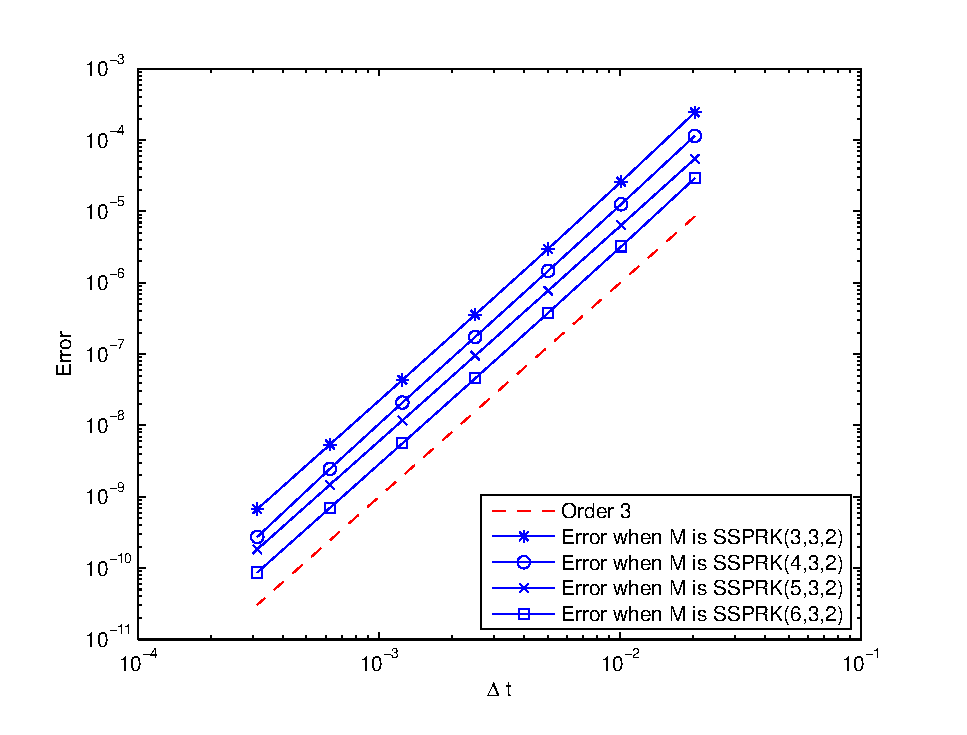
\includegraphics[width=0.5\textwidth]{Pictures/convergence_3rd_ord}%
    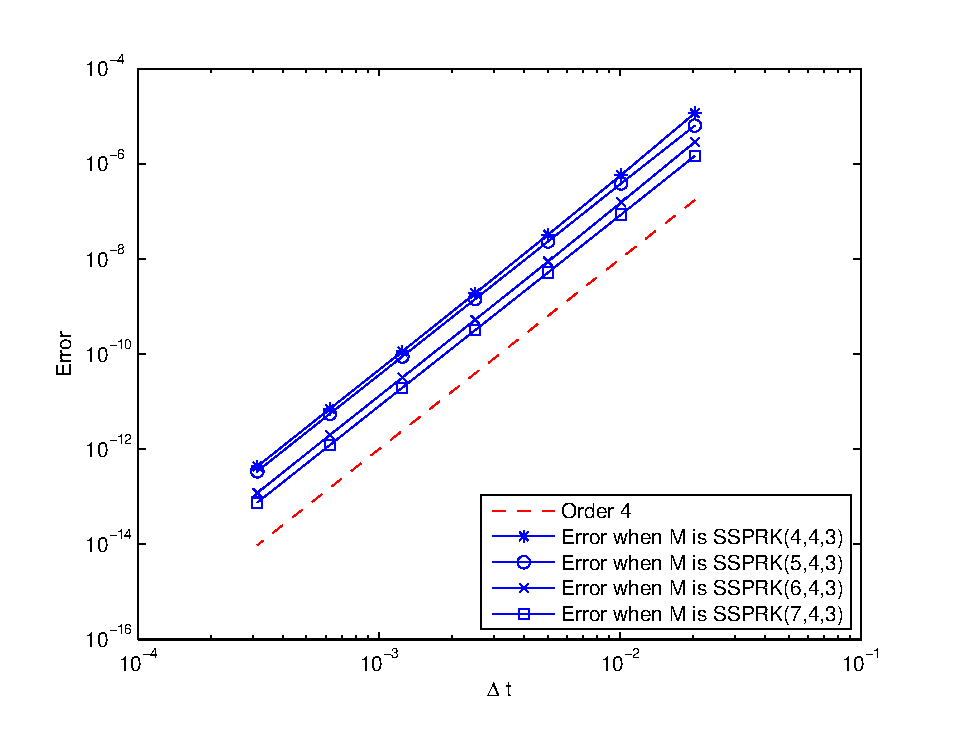
\includegraphics[width=0.5\textwidth]{Pictures/convergence_4th_ord_(2)}
    \caption{Convergence of $TM^{n-2}R$ Runge-Kutta scheme when (a) $M$ is SSPRK($s $,$ 4 $,$ 2 $) method and (b) $ M $ is SSPRK($ s $,$ 4 $,$ 3 $) method.}
    \label{fig5.2}
\end{figure}

\subsection{Application to nonlinear problems}\label{subsec:nonlinear_problems}

\subsubsection{Burger's equation}\label{subsubsec:burgers}

The inviscid Burger's equation consists of the hyperbolic conservation law
\begin{equation}\label{eq5.5}
    U_{t} + f(U)_{x} = 0,
\end{equation}
when the flux function $f(U) = \frac{1}{2}U^{2}$. We consider initial data
\begin{equation}\label{eq5.6}
    u(0,x)  = \frac{1}{2} - \frac{1}{4}sin{\pi x},
\end{equation}
on a periodic domain $x \in [0,2)$. The solution advances to the right where it eventually exhibits a shock. We perform a semi-discetisation of $f(U)_{x}$ using an upwind approximation \cite{Ketcheson2009} that gives
\begin{equation}\label{eq5.7}
    f(U)_{x} \approx \frac{1}{\Dt}\bigl(f(u_{i}) - f(u_{i-1})\bigr).
\end{equation}

The above time discretisation is SSP when coupled with Forward Euler method under time restriction $\Dt \leq {\Dt}_{FE} = \frac{\Delta x}{\|u(0,x)\|_{\infty}}$. We integrate to time $t_{f} = 2.3$ with $m = 256$ points in space.
\newline

\begin{figure}[t!]
    \centering
    \subfloat[$\sigma = 6.0$]{\label{fig5.3a}%
      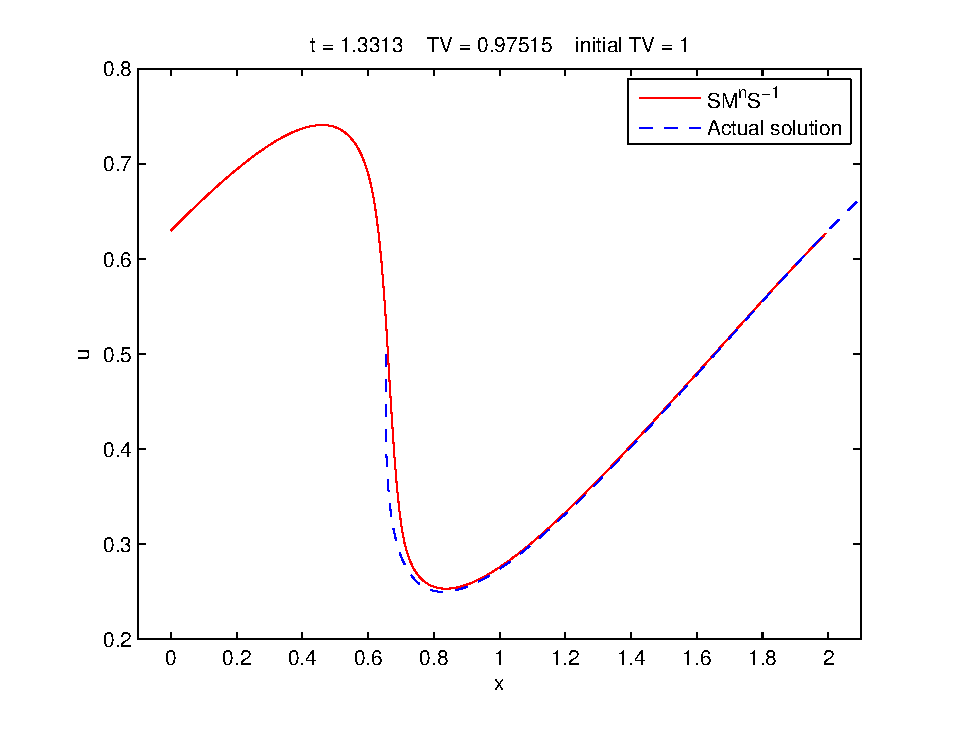
\includegraphics[width=0.5\textwidth]{Pictures/burgers_cont_tvd}}%
    \subfloat[$\sigma = 7.1$]{\label{fig5.3b}%
      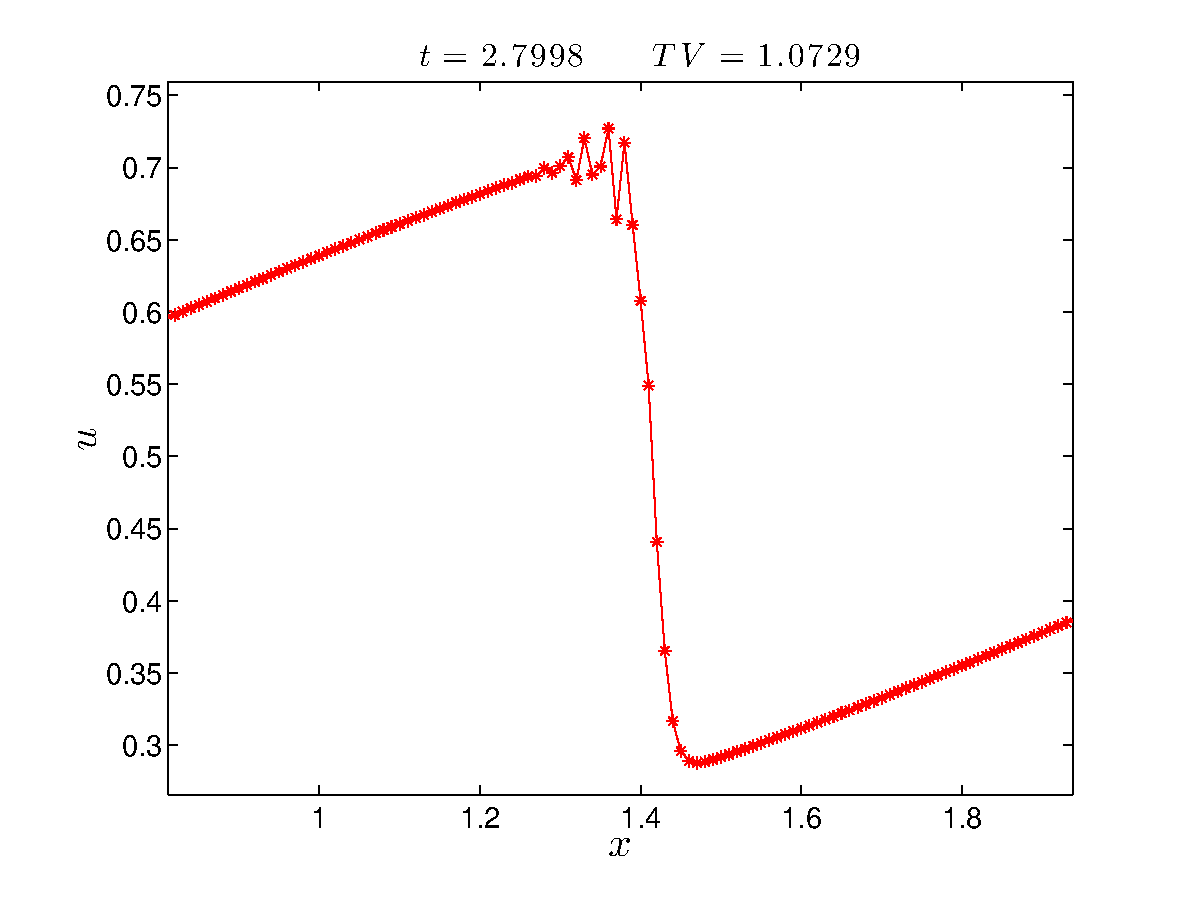
\includegraphics[width=0.5\textwidth]{Pictures/burgers_cont_no_tvd}}
    \caption{Solution of Burger's equation with continuous initial data, using a $ TM^{n-2}R $ scheme, where $ M $ is SSPRK($ 10 $,$ 4 $,$ 3 $). The SSP coefficient is $ c = 6.0 $.}
    \label{fig5.3}
\end{figure}

Burger's equation was solved using an ESSPRK-scheme with time-step restriction $\Dt \leq \sigma{\Dt}_{FE}$, where $\sigma$ indicates the size of the time step. Figure \ref{fig5.3} shows that if $\sigma$ stays below the SSP coefficient of the method $M$, then no oscillations are observed. If this stability limit is violated, then oscillations appear. \yianniscomment{Elaborate more: Sharpness of SSP coefficient} We were able to determine when exactly the nonlinear stability is not satisfied by computing the the total-variation (TV) norm at each step of the computation process. This indicates that the ESSPRK-scheme inherits the time-step restriction from the SSP coefficient of the main method $M$.
\newline

We also consider Burger's equation with discontinuous data
\begin{equation}\label{eq5.8}
    u(0,x)  = \left\{
                \begin{array}{ll}
                  1, & \hbox{$0.5 \leq x \leq 1.5$} \\
                  0, & \hbox{otherwise.}
                \end{array}
              \right.
\end{equation}

Figure \ref{fig5.4} shows the result of solving the discontinuous problem using anESSPRK-scheme, with $M$ an SSPRK($4$,$4$,$3$). Clearly, the monotonicity in the TV-norm is violated at $t = 0$ because the method $S$ is not an SSP method. However, this does not propagate in time if the time-step size $\sigma$ is kept below the SSP coefficient of method $M$. Otherwise, oscillations continue to appear for $t > 0$. The actual solution was plotted using the method of the characteristics and is given by

\begin{equation}\label{eq5.9}
    u(t,x)  = \left\{
                \begin{array}{ll}
                  0, & \hbox{$0 \leq x \leq 0.5$} \\
                  \frac{x-0.5}{t}, & \hbox{$0.5 < x \leq 0.5 + t$} \\
                  1, & \hbox{$0.5 + t < x \leq 1.5  + \frac{t}{2}$} \\
                  0, & \hbox{$1.5  + \frac{t}{2} < x \leq 2$}. \\
                \end{array}
              \right.
\end{equation}

\begin{figure}[t!]
    \centering
    \subfloat[$\sigma = 1.97$]{\label{fig5.4a}%
      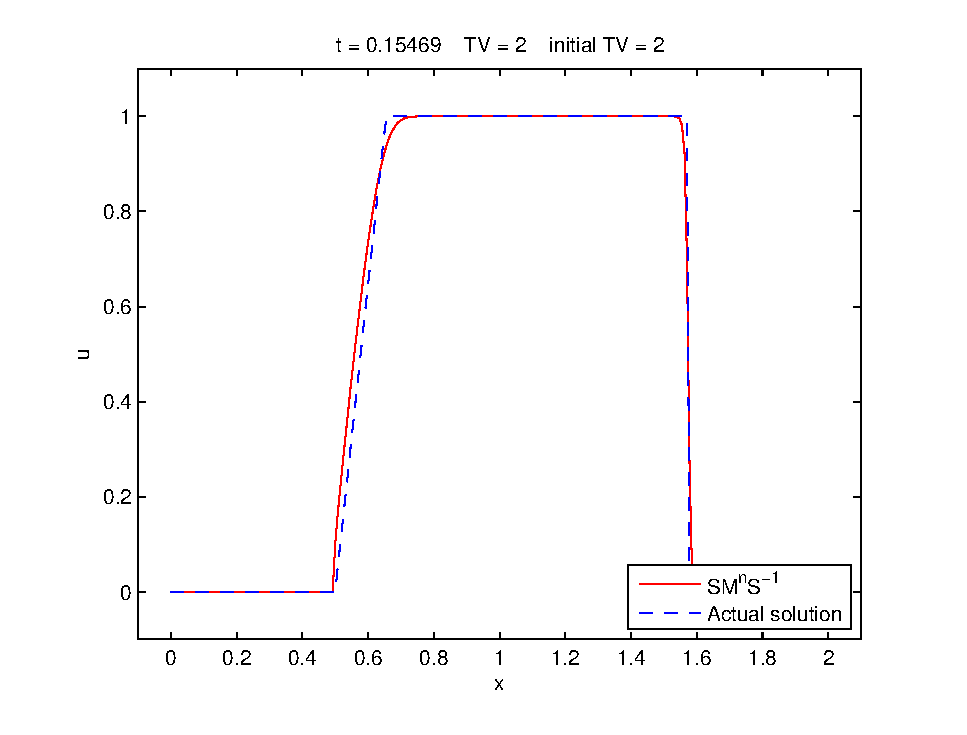
\includegraphics[width=0.5\textwidth]{Pictures/burgers_discont_tvd.eps}}%
    \subfloat[$\sigma = 2.2$]{\label{fig5.4b}%
      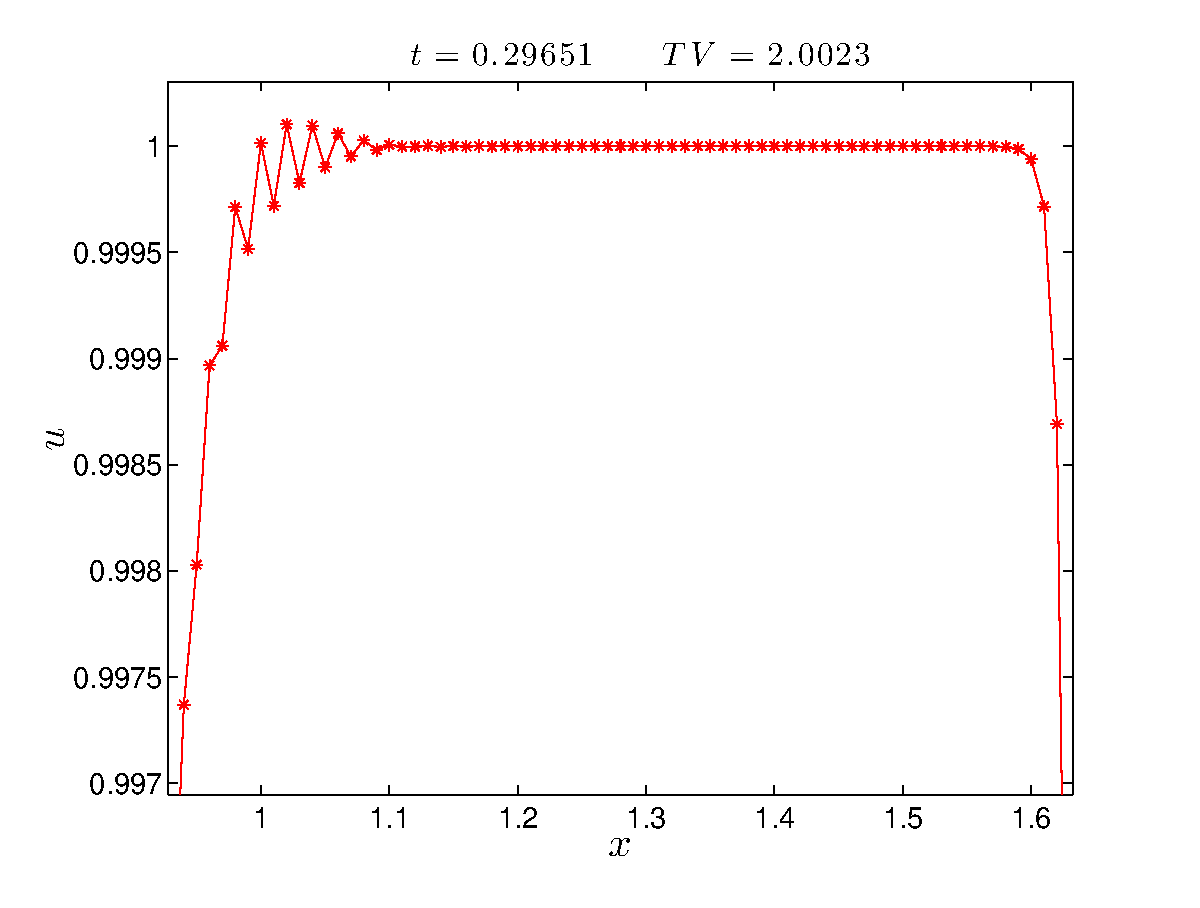
\includegraphics[width=0.5\textwidth]{Pictures/burgers_discont_no_tvd.eps}}
    \caption{Solution of Burger's equation with discontinuous initial data, using a $ TM^{n}R $ scheme, where $ M $ is SSPRK($ 5 $,$ 4 $,$ 2 $) method. The SSP coefficient is $ c = 1.97 $.}
    \label{fig5.4}
\end{figure}

\subsubsection{Buckley-Leverett equation}\label{subsubsec:B-L}

	\section{Conclusions}\label{sec:Conclusion}
We used the theory of strong stability preserving time discretizations
with Butcher's algebraic interpretation of order to construct
effective order SSP Runge--Kutta (ESSPRK) methods. 
These methods, when accompanied by starting and stopping
schemes, attain an order of accuracy higher than their (classical) order.
We proposed a new choice of starting and stopping methods to allow the
overall procedure to be SSP.
We proved that explicit Runge--Kutta methods with strictly positive 
weights have at most effective order four. 
This extends the barrier already known in the case of classical order
explicit SSPRK methods.

ESSPRK methods of effective order three and four
were constructed by numerical optimization.
Most of the methods found were optimal because they achieved
the upper bound on the SSP coefficient known from linear
problems.
Also, despite the non-existence of four-stage, four-order explicit SSPRK methods, 
we found effective order four methods with four stages (of classical 
order two and three). 


We performed numerical tests which confirmed the accuracy and
SSP properties of the ESSPRK methods.
Interestingly, compared to what is observed with standard SSPRK schemes,
there was much closer agreement between the (theoretical) stability limit
given by the SSP coefficient and that observed in practice
(e.g., when measuring total variation of solutions of Burgers' equation).

The ideas here were applied to explicit Runge--Kutta methods, but they
could also be applied to other classes of methods including implicit
Runge--Kutta methods, general linear methods, and Rosenbrock methods.


	%\section*{Acknowledgments}{
	%The second author thanks Jim Verner for introducing him to this
	%problem and for his support over the years.
	%}

	%%% Appendix and Bibliography %%%
	%\appendix
	%% appendix A
\section{Proofs}\label{appendixA}

%\subsection{Proof of Lemma~\ref{Davids_lemma}}

% \begin{lem}\label{lemA.1}
%     Given \( b,v \in \mathbb{R}^{n} \), suppose that
%     \begin{subequations}\label{eq4.3}
%         \begin{align}
%             b_i & > 0 \mbox{ for all } i, \label{eq4.3a} \\
%             \sum_{i=1}^n b_i & = 1, \label{eq4.3b} \\
%             \sum_{i=1}^n b_i v_i^2 & = \left(\sum_{i=1}^n b_i v_i \right)^2. \label{eq4.3c}
%         \end{align}
%     \end{subequations}
%     Then all \(v_i\) are equal but at most one; in other words, there exists \( \alpha\in\mathbb{R} \) and an integer \(k\) such that \(v_i=\alpha\) for all \(i\ne k\).
% \end{lem}
% \colintodo{decide whether to state lemma here or in text: not both}%
\begin{proof}[Proof of Lemma~\ref{Davids_lemma}]
    Let \( k \) be an arbitrary integer between \( 1 \) and \( n \). Then by collecting terms in powers of \( v_k \),
%\eqref{eq4.3c} can be written
\eqref{eq:DavidsLemma_c} can be written
\begin{equation*}
    %b_k v_k^2 + \sum_{i\ne k} b_i v_i^2 - b_k^2 v_k^2 - 2 b_k v_k \sum_{i\ne k} b_i v_i
    %        - \left(\sum_{i\ne k} b_i v_i \right)^2 = 0 \\
  b_{k}(1-b_{k})v_{k}^{2} - 2b_{k}v_{k}\sum_{i \neq k}b_{i}v_{i} + \sum_{i \neq k}b_{i}v_{i}^{2} - \left(\sum_{i \neq k}b_{i}v_{i}\right)^{2} = 0.
\end{equation*}
This is a quadratic equation in \( v_{k} \) whose roots are real if and only if
\begin{equation*}
    4b_{k}^{2}\left(\sum_{i \neq k}b_{i}v_{i}\right)^{2} - 4b_{k}(1-b_{k})\left(\sum_{i \neq k}b_{i}v_{i}^{2} - \left(\sum_{i \neq k}b_{i}v_{i}\right)^{2}\right) \geq 0.
\end{equation*}
Expanding and canceling terms yields
\begin{equation*}
    (1-b_{k})\sum_{i \neq k}b_{i}v_{i}^{2} - \left(\sum_{i \neq k}b_{i}v_{i} \right)^{2} \leq 0.
\end{equation*}
By \eqref{eq:DavidsLemma_b}, \( 1-b_{k} = \sum_{j \ne k}b_{j} \), so we have
\begin{equation*}
    \sum_{j \neq k}b_{j}\sum_{i \neq k}b_{i}v_{i}^{2} - \sum_{j \neq k}b_{j}v_{j}\sum_{i \neq k}b_{i}v_{i}.
\end{equation*}
Noting that the terms corresponding to \( i = j \) in the two double sums cancel gives
\begin{equation*}
    \sum_{j \neq k}b_{j}\sum_{i \neq k,j}b_{i}v_{i}^{2} - \sum_{j \neq k}b_{j}v_{j}\sum_{i \neq j,k}b_{i}v_{i} \leq 0,
\end{equation*}
or
\begin{equation*}
    \sum_{j \neq k}b_{j}\sum_{i \neq k,j}b_{i}v_{i}(v_{i} - v_{j}) \leq 0.
\end{equation*}
Adding the left hand side to itself, but with \( i,j \) reversed, yields
\begin{equation*}
    \sum_{j \neq k}b_{j}\sum_{i \neq k,j}b_{i}v_{i}(v_{i} - v_{j}) - \sum_{i \neq k}b_{i}\sum_{j \neq k,i}b_{j}v_{j}(v_{i} - v_{j}) \leq 0.
\end{equation*}
This simplifies to
\begin{equation*}
    \sum_{j \neq k}\sum_{i \neq k,j}b_{j}b_{i}(v_{i} - v_{j})^{2} \leq 0.
\end{equation*}
By \eqref{eq:DavidsLemma_a}, this can only hold if \( v_{i} = v_{j} \) for all \( i,j \neq k \).
\end{proof}

%\subsection{Proof of Theorem~\ref{thm:positiveb}}

\begin{proof}[Proof of Theorem~\ref{thm:positiveb}]
    Consider the fifth-effective order conditions of classical order two for the main method, listed in Table~\ref{tab:Effective_oc}. We declare \( \beta_{2} \) as a free parameter and we treat the case that \( \beta_{2} \) is nonzero separately from the one that is zero. Among others the order conditions must satisfy the following equations:
    \begin{subequations}\label{eq4.4}
        \begin{align}
            \bm{b}^{T}\bm{e} &= 1 \label{eq4.4a} \\
            \bm{b}^{T}A\bm{c} &= \frac{1}{6} \label{eq4.4b} \\
            \frac{1}{2}\bm{b}^{T}\bm{c}^{2} - \frac{1}{6} &= \beta_{2} \label{eq4.4c} \\
            \frac{1}{4}\bm{b}^{T}\bm{c}^{4} - \bm{b}^{T}C^{2}A\bm{c} + \bm{b}^{T}(A\bm{c})^{2} &= \beta_{2}^{2}, \label{eq4.4d}
        \end{align}
    \end{subequations}
    where the powers on vectors are understood component-wise. Supposing that the above equations can be solved simultaneously, then substituting \eqref{eq4.4b} in \eqref{eq4.4c} and collecting terms gives \( \beta_{2} = \bm{b}^{T}\bm{v} \), where \( \bm{v} = \frac{1}{2}\bm{c}^{2} - A\bm{c} \). Squaring yields
    \begin{equation*}%\label{eq4.5}
        \beta_{2}^{2} = \bm{b}^{T}\Bigl(\frac{1}{2}\bm{b}^{T}\bm{c}^{2} - \frac{1}{6}\Bigr)\Bigl(\frac{1}{2}\bm{c}^{2} - A\bm{c}\Bigr),
    \end{equation*}
    %Rewriting \eqref{eq4.4d} and subtracting from \eqref{eq4.5} gives
    and subtracting \eqref{eq4.4d} gives
    \begin{equation*}
        \bm{b}^{T}\biggl(\Bigl(\frac{1}{2}\bm{c}^{2} - A\bm{c}\Bigr)^{2} - \Bigl(\frac{1}{2}\bm{b}^{T}\bm{c}^{2} - \frac{1}{6}\Bigr)\Bigl(\frac{1}{2}\bm{c}^{2} - A\bm{c}\Bigr)\biggr) = 0.
    \end{equation*}
    Defining \( \bm{w} = \bm{v}^{2} - \beta_{2}\bm{v} \), this can be written as
    \begin{equation}\label{eq4.6}
        \bm{b}^{T}\bm{w} = 0.
    \end{equation}
    Now, if we require \( b_{i} > 0 \) for all \( i \in \{1,\dots, s\} \), then \eqref{eq4.6} is satisfied if \( \bm{w} = \bm{0} \),
or if there is a least one negative and at least one positive element in \( \bm{w} \).
We will show that neither can be true.


\paragraph{Case 1: \( \bm{w} = \bm{0}, \beta_2 \neq 0 \).}

Here \( v_{i}^{2} - \beta_{2}v_{i} = 0 \) for all \( i \in \{1,\dots,s\} \), so either \( v_{i} = 0 \) or \( v_{i} = \beta_{2} \).
The case that \( \bm{v} = 0 \) is equivalent with a Runge-Kutta method to have stage order two. This means that for a particular time \( t = t^{n} + c_{i}\Delta t \), for \( i \in \{1, \dots, s\} \), the stage \( \textbf{Y}_{i} \) will be at least a second order approximation to the solution at that time.
For an explicit Runge-Kutta method, the stage \( \textbf{Y}_{2} = \bm{u}^{n} + \Dt\bm{F}(\bm{u}^{n}) \) can not have stage order more than one, hence not all the components of \( \bm{v} \) are zero. Also, \( v_{1} = 0 \) because the first row of matrix \( A \) has only zeros. Let \( I = \{ i \;|\; v_{i} = \beta_{2}, \; i = 1,\dots,s \} \) and \( v_{j} = 0 \) if \( j \neq I \). Then, by using \eqref{eq4.4a} \( \beta_{2} = \sum_{i=1}^{s}b_{i}v_{i} = \sum_{i \in I}b_{i}\beta_{2} = \beta_{2}\sum_{i \in I}b_{i} < \beta_{2} \). Therefore a contradiction.


\paragraph{Case 2: \( \bm{w} \neq \bm{0}, \beta_2 \neq 0 \).}

    Then, there exists at least one component \( w_{i} = v_{i}^{2} - \beta_{2}v_{i} \) such that \( w_{i} < 0 \) and at least one component \( w_{j} = v_{j}^{2} - \beta_{2}v_{j} \) such that \( w_{j} > 0 \). We will show that \( 0 < v_{i} < \beta_{2} < v_{j} \).

    Consider first the component \( w_{i} \). If \( w_{i} < 0 \), then \( v_{i}^{2} < \beta_{2}v_{i} \). Therefore,
    \begin{equation}\label{eq4.7}
        (\beta_{2})^{2} = \sum_{j=1}^{s}b_{j}v_{j}^{2} < \sum_{j \neq i}^{s}b_{j}v_{j}^{2} + b_{i}\beta_{2}v_{i}.
    \end{equation}
    The inequality \eqref{eq4.7} can be written as
    \begin{equation}\label{eq4.8}
        \begin{split}
            \beta_{2}\sum_{j=1}^{s}b_{j}v_{j} &< \sum_{j \neq i}^{s}b_{j}v_{j}^{2} + \beta_{2}b_{i}v_{i} \\
            \beta_{2}\sum_{j \neq i}^{s}b_{j}v_{j} &< \sum_{j \neq i}^{s}b_{j}v_{j}^{2} \\
            \beta_{2}\sum_{j \neq i}^{s}b_{j}v_{j} &< (\beta_{2})^{2}.
        \end{split}
    \end{equation}
    Suppose that \( v_{i} < 0 \). Then
    \begin{equation*}
        \beta_{2} = \sum_{j=1}^{s}b_{j}v_{j} < \sum_{j \neq i}^{s}b_{j}v_{j}
    \end{equation*}
    From \eqref{eq4.8} we have
    \begin{equation*}
            \beta_{2}\beta_{2} < \beta_{2}\sum_{j \neq i}^{s}b_{j}v_{j} < (\beta_{2})^{2},
    \end{equation*}
    which gives a contradiction. Since \( v_{i} \neq 0 \), then \( v_{i} > 0 \) and in this case \( 0 < v_{i} < \beta_{2} \).

    Now consider the component \( w_{j} = v_{j}^{2} - \beta_{2}v_{j} \). Since \( w_{j} > 0 \), then \( v_{j}^{2} > \beta_{2}v_{j} \). If \( v_{j} < 0 \), then \( v_{j} < \beta_{2} \) and \( v_{j} < 0 < v_{i} < \beta_{2} \). Hence \( \beta_{2} \) is larger than all components of \( \bm{v} \). This leads to a contradiction since
    \begin{equation*}
            \beta_{2} = \sum_{k=1}^{s}b_{k}v_{k} < \sum_{k=1}^{s}b_{k}\beta_{2} < \beta_{2}.
    \end{equation*}
    As before \( v_{j} \) can no be zero, therefore \( v_{j} > 0 \) which gives \( v_{j} > \beta_{2} \).

    In total we have
    \begin{equation}\label{eq4.9}
        v_{1} = 0 \quad \text{ and } \quad 0 < v_{i} < \beta_{2} < v_{j}, \text{ for } i,j \in \{2,\dots,s\}.
    \end{equation}
    However, based on Lemma~\ref{Davids_lemma} all \( v_{i} \) must be equal except form one. Let that component be \( v_{k} \). If \( k = 1 \), then \( v_{i} = \delta \) for \( i,j \in \{2,\dots,s\} \). If \( k \neq 1 \), then \( v_{i} = 0 \) for \( i \in \{2,\dots,s\}\setminus\{k\} \). Both cases contradict with \eqref{eq4.9}. Thus, the equations \eqref{eq4.4} can not be solved simultaneously and no five-effective order Runge-Kutta of classical order two exists with positive weights.


    \paragraph{Case 3: \( \beta_2 = 0 \).}
    \colintodo{Ok to label this as third case?}
    %In the case that \( \beta_{2} = 0 \) then
    Here \eqref{eq4.4d} becomes
    \begin{equation*}
        \frac{1}{4}\bm{b}^{T}\bm{c}^{4} - \bm{b}^{T}C^{2}A\bm{c} + \bm{b}^{T}(A\bm{c})^{2} = 0,
    \end{equation*}
    or equivalently
    \begin{equation*}
        \bm{b}^{T}\bm{v}^{2} = 0.
    \end{equation*}
    Since \( \bm{v} \) can not be identical equal to zero, it must have a nonzero component. But since \( \bm{b} > 0 \), then \( \bm{b}^{T}\bm{v}^{2} > 0 \). Immediately this prevents the existence of five-effective order Runge-Kutta of classical order greater than two if we require positive weights.
\end{proof}
	\bibliographystyle{acm} %apalike
	\bibliography{bibliography2}

\end{document}
